% ============================================================================
%  Risk-Driven UAV Swarm Patrol for Fast Road Accident Detection
%  M51 Khalde-Awali corridor, Lebanon
%
%  Single-file Overleaf source. Every figure is drawn with TikZ / pgfplots,
%  so there are no external image files to upload. Compile with pdfLaTeX.
% ============================================================================
\documentclass[11pt]{article}

\usepackage[a4paper,margin=2.6cm]{geometry}
\usepackage[T1]{fontenc}
\usepackage[utf8]{inputenc}
\usepackage{lmodern}
\usepackage{amsmath,amssymb}
\usepackage{booktabs}
\usepackage{array}
\usepackage{caption}
\usepackage{tikz}
\usepackage{pgfplots}
\usepackage{enumitem}
\usepackage[hidelinks]{hyperref}

\pgfplotsset{compat=1.18}
\usetikzlibrary{arrows.meta,positioning,calc}

\captionsetup{font=small}
\captionsetup[table]{position=top,skip=4pt}

% Let floats sit closer to where they are cited
\renewcommand{\topfraction}{0.9}
\renewcommand{\bottomfraction}{0.8}
\renewcommand{\textfraction}{0.07}
\renewcommand{\floatpagefraction}{0.8}

% Colours
\definecolor{polUniform}{RGB}{29,78,216}
\definecolor{polRisk}{RGB}{234,88,12}
\definecolor{barBlue}{RGB}{63,81,181}
\definecolor{boxData}{RGB}{237,237,237}
\definecolor{boxModel}{RGB}{219,226,247}
\definecolor{boxSim}{RGB}{222,240,224}

\title{Risk-Driven UAV Swarm Patrol for Fast Road Accident Detection
on the M51 Corridor, Lebanon}

\author{%
  Hussein Nasereddine$^{1}$, Walid Chaar$^{2}$, and Ali Kalakech$^{3}$\\[6pt]
  {\small $^{1}$Independent Research Engineer, Beirut, Lebanon}\\
  {\small $^{2}$Research Department, Novum Research, Beirut, Lebanon}\\
  {\small $^{3}$Engineering Department, Lebanese International University, Beirut, Lebanon}\\
  {\small Corresponding author: husseinnaserddine21@gmail.com}}

\date{Version 1.0, September 2026}

\begin{document}
\maketitle

% ===========================================================================
\begin{abstract}
\noindent
When a crash happens on a motorway without automatic incident detection, help
can only start once someone reports it. This paper studies how a swarm of
patrol drones can detect crashes faster on the 28.6~km Khalde--Awali section of
the M51 motorway in Lebanon, and where along the road the drones should fly.
IoT sensors are mounted on the guardrail along the side of the road. When a
crash happens, the sensor at the crash site sends a short-range radio alert,
and a drone detects the crash when its patrol brings it within range of that
alert. To decide where the drones should patrol, we built a crash-rate model
from two main datasets: 1{,}152 ambulance-attended crashes recorded by the
Lebanese Red Cross over 31 months (2016--2018), and GPS traffic data from the
\emph{tari2ak} smartphone application, obtained through a collaboration with
the National Council for Scientific Research in Lebanon (CNRS-L). The ambulance records give only the
name of a town, not an exact location, so we modelled crashes in seven road
regions and five time slots per day and fitted a Poisson regression with an
exposure offset to 1{,}085 region--month--time-slot cells. The model gives the
expected number of crashes per kilometre per hour for each region and time
slot. Roadside activity, measured as roadside landmarks per kilometre, is the
strongest risk factor (rate ratio 3.84), and the predicted regional crash
totals agree closely with the observed ones (correlation 0.990). A simulator
uses these rates to create crashes and to divide the road among the drones so
that each drone covers the same expected number of crashes. Over 50 simulated
30-day periods per fleet size, this risk-aware plan cut the average alert time
with ten drones from 177~s to 140~s compared with equal-length segments, and
detected 80\% of crashes within two minutes with about 19 drones instead of
about 21. It also has a cost: it left a long, quiet stretch in the south that
one drone could not cover in time, so with 13 drones it missed 7.7\% of
crashes while equal-length segments missed none. All detection results come
from simulation; no field trials have been run yet.
\end{abstract}

\noindent\textbf{Keywords:} UAV swarm; road accident detection; crash-frequency
model; Poisson regression; patrol allocation; IoT alert; guardrail sensor;
Lebanon

% ===========================================================================
\section{Introduction}

\subsection{Background and Context}

Road crashes kill about 1.19 million people every year. About 92\% of these
deaths happen in low- and middle-income countries, even though these countries
have only about 60\% of the world's vehicles~\cite{who2023}. Lebanon is one of
these countries. Its coastal motorways combine high speeds with shops, fuel
stations and beach resorts that open directly onto the road. Drivers slow down,
turn and stop in the middle of fast traffic.

Some parts of this problem take a long time to fix. Rebuilding a road takes
years, and changing how people drive takes even longer. One part, however, is
both important and quick to improve: the time it takes for anyone to learn that
a crash has happened. Medical studies show why this matters. In more than
1{,}400 crashes on Spanish roads, a medical response that was ten minutes
faster was linked to about a one-third lower chance of death~\cite{sanchez2010}.
In a study of 2{,}268 counties in the United States, counties where the
ambulance took 12 minutes or more had a crash death rate 1.46 times higher than
counties where it took less than 7 minutes~\cite{byrne2019}. Help cannot start
before the crash is detected, so detection is the first step in this chain.

On a road without cameras or automatic crash detection, the alert usually
depends on a passing driver making a phone call. This is slow and unreliable.
Our system removes this human step in two parts. First, small IoT sensors are
mounted on the guardrail (the metal crash barrier) that runs along the side of
the road. When a crash happens, the sensor at that point detects it and sends a
short-range radio alert. Second, patrolling unmanned aerial vehicles (UAVs), or
drones, pick up this alert when they fly close enough to the sensor. A swarm of
such drones, each one responsible for its own stretch of road, turns detection
into a coverage problem: how many drones do we need, where should they fly, and
how quickly will the first one hear the alert?

\subsection{Research Problem and Knowledge Gap}

Any system of this kind must decide where to put its drones. To do this, it
needs a model of where and when crashes happen.

In practice, most systems use an expert score. Traffic, road curves and merging
are each given a small score, such as 0, 1 or 2, by hand. The scores are then
added together using weights that the analyst chooses, and the result is called
``risk''. Such a score has three serious problems. It has no units, so scores
on different roads cannot be compared. It cannot be checked, because nothing
you can measure on the road corresponds to a score of 1.4. And it says nothing
about how many crashes happen, only which places are riskier than others, so
the yearly number of crashes has to be assumed separately.

Research on drones has the opposite gap. Studies of multi-robot patrolling are
advanced, but they usually assume that every point on the route is equally
important~\cite{elmaliach2009,portugal2011}. Reviews of drones in road safety
describe many uses, but rarely explain the model that decides where the drones
actually go~\cite{outay2020,menouar2017}.

\textbf{The gap this paper addresses} lies between these two areas. We ask what
changes in a drone patrol system when the hand-made risk score is replaced by a
crash rate that is estimated from real crash records, has real units, and can
be checked against data.

\subsection{Research Objectives}

This study has five objectives: (i) to build a crash-rate model for the
corridor at the finest level of detail that the crash records allow; (ii) to
use only this model to create simulated crashes in time and space; (iii) to
build two ways of placing the drones, one that ignores risk and one that gives
each drone the same expected number of crashes; (iv) to model how a drone
detects a crash through a short-range radio alert sent by a guardrail-mounted
sensor, using realistic drone speeds and radio ranges; and (v) to measure,
through repeated simulation, how the alert time, the share of crashes found
within two minutes, and the share of missed crashes change with the number of
drones.

\subsection{Main Focus}

The main focus is the risk model and its effect on the drone swarm. We ask four
questions. What does a fitted crash-rate model look like on this road, and which
factors drive it? Does it agree with the crash counts we observed? When it
replaces an expert score in a working patrol simulator, do the drones fly
differently? And does this change help detection, both on average and in the
worst case?

\subsection{Main Contribution}

This study makes four contributions: (i) a complete description of a drone
swarm system for crash detection whose risk model is a fitted crash rate, not
a score, including every step that turns the model's output into patrol
segments; (ii) evidence that, on this road, roadside activity matters more than
road shape, and that the resulting pattern of risk is the opposite of what the
expert score assumed; (iii) a fair comparison of two patrol plans at the real
crash rate of the road, reporting both the average result and the worst case;
and (iv) a clear negative result: the risk-aware plan improves the average and
the two-minute target, but misses more crashes for some fleet sizes, because
it gives each drone an equal number of crashes rather than an equal length of
road.

\subsection{Overview of Methodology}

The model rests on two main datasets. The first is the ambulance dispatch
records of the Lebanese Red Cross, which give the crash counts. The second is a
GPS dataset collected by the \emph{tari2ak} smartphone application running in
moving vehicles, which we obtained through a collaboration with the National
Council for Scientific Research in Lebanon (CNRS-L), which gives the traffic level and speeds. We added road
geometry from OpenStreetMap and weather data, and combined everything into one
table of 1{,}085 cells: 7 regions $\times$ 31 months $\times$ 5 time slots per
day. We fitted a Poisson regression model to this table, with an exposure term
for road length and time. We then turned the model's predictions into a table
of crash rates per kilometre per hour, one for each region and time slot. A
simulator uses this table to create crashes, split the road into patrol
segments, fly the drones back and forth along their segments, and measure how
long it takes until the first drone receives the alert sent by the
guardrail-mounted sensor at each crash. We repeated this for fleets of 1 to 30
drones under both patrol plans.

% ===========================================================================
\section{Literature Review}

\subsection{Theoretical Concepts}

\paragraph{Counting Crashes.}
Crash studies count how many crashes happen on a stretch of road over a period
of time. If $Y_{it}$ is the number of crashes on stretch $i$ in period $t$, the
standard model is
$E[Y_{it}] = E_{it}\exp(\mathbf{x}_{it}'\boldsymbol{\beta})$. Here
$E_{it}$ is the \emph{exposure}, for example road length multiplied by time, and
$\mathbf{x}_{it}$ holds the factors that may affect risk. Including exposure in
this way turns a count into a rate, so that a long stretch observed for a long
time can be compared fairly with a short stretch observed for a short
time~\cite{washington2020}. A common question is whether to use a Poisson model
or a negative binomial model. Crash counts often vary more than a Poisson model
expects (\emph{overdispersion}), and ignoring this makes results look more
certain than they are~\cite{lordmannering2010,miaou1994}. The right test,
however, is whether this extra variation remains \emph{after} the risk factors
and exposure are in the model, not whether it exists in the raw
counts~\cite{cameron1990,lord2005}.

\paragraph{Patrolling.}
A patrol problem asks how a team of agents should move so that every point in
an area is visited often enough. Classic methods try to keep the time between
two visits to any point as short as possible. Most of them assume that every
point is equally important~\cite{elmaliach2009,portugal2011}. Some methods give
points different weights, but the weights are usually chosen, not measured.

\paragraph{Detection Time.}
Once a crash has happened at a known place, and a drone flies back and forth
over its stretch at a constant speed, the time until the drone reaches the
crash can be calculated exactly from the drone's position and direction. The
only random parts are where and when the crash happens. This is why an accurate
crash model matters more here than a detailed flight model: the flight is
simple, but the crashes are not.

\subsection{Previous Studies and Existing Methodologies}

The Highway Safety Manual gives a standard two-step method. A \emph{safety
performance function} predicts crashes on a road under normal conditions, and
\emph{crash modification factors} adjust the prediction for differences from
those conditions~\cite{hsm2010}. Versions for motorways were developed in NCHRP
Project 17-45~\cite{bonneson2012}, and the effect of ramps and other motorway
design features was measured by Park, Fitzpatrick and Lord~\cite{park2010}.
Empirical Bayes methods correct for a common statistical trap in before-and-after
studies~\cite{hauer1997}. A known concern is that these models do not always
work in a new place: Elvik showed that the effect of road curves varies a lot
from one country to another~\cite{elvik2013}. Mannering and Bhat review the
wider range of methods~\cite{mannering2014}.

For drones, Kanistras et al.\ reviewed early work on traffic
monitoring~\cite{kanistras2013}, Menouar et al.\ described how drones fit into
smart transport systems~\cite{menouar2017}, and Outay, Mengash and Adnan
reviewed drone uses in road safety, traffic and road maintenance, including
crash-site work~\cite{outay2020}. Mozaffari et al.\ explain how drones
communicate in wireless networks~\cite{mozaffari2019}, and Erdelj et al.\
describe how drones support disaster response~\cite{erdelj2017}.

The alert itself also has a body of research. LoRa is a low-power, long-range
radio often used for small battery-powered sensors. Field tests measured ranges
of a few kilometres in towns and about 15~km in open land~\cite{petajajarvi2015}.
Several prototypes connect a motion or tilt sensor to a LoRa radio to send an
automatic crash alert~\cite{vinodhini2025}. In our system, the sensors are
fixed to the roadside guardrail, and the drones act as moving receivers that
pick up the alert as they fly past.

\subsection{Research Gaps}

Three gaps motivate this work.

\textbf{First, drone patrol systems rarely explain their risk model.} Papers
describe the patrol method in detail but the risk weights in a sentence. They
rarely say where the weights come from or whether they match real crash counts.

\textbf{Second, crash records without exact locations are rarely studied.} Most
crash studies assume that every crash can be placed on a map. When records come
from ambulance dispatch rather than police reports, the location may be only
the name of a town. There are few methods for this case, and the usual answer,
an expert score, is rarely compared with a fitted model.

\textbf{Third, patrol studies report averages.} Most studies report the average
detection time. A plan that puts more drones on busy stretches can improve the
average while leaving a quiet stretch almost unwatched, and the average does
not show this.

\subsection{Positioning of the Present Study}

This study connects crash modelling with the planning of patrol resources. It
does not propose a new statistical method or a new patrol algorithm. Its aim is
to link the two with a documented and checked crash-rate model, and to report
openly what this link gains and what it costs.

% ===========================================================================
\section{Materials and Methods}

\subsection{Study Area}

The study road is the northern part of the M51 South Coastal Highway
(\emph{Autostrade el-Janoub}). It runs south from the Khalde interchange
($33.7780^{\circ}$N, $35.4904^{\circ}$E), just south of Beirut Rafic Hariri
International Airport, to the Awali River bridge ($33.5963^{\circ}$N,
$35.3727^{\circ}$E), north of Saida. Its length measured along the centre of
the road, called the \emph{chainage}, is 28.6002~km. The Awali River marks the
border between Mount Lebanon and South Governorate, which makes it a natural
end point.

The road has two to three lanes in each direction and a speed limit of 80~km/h.
The speed below which 85\% of drivers travel ranges from 79.4 to 113.4~km/h.
About 200{,}000 vehicles a day enter Greater Beirut through the southern
entrance at Khalde~\cite{worldbank2017}. Traffic drops further south as cars
leave at the exits, giving an average of about 90{,}000 vehicles a day along
the study road. Access to the road is poorly controlled: nineteen interchanges
and many small entrances serve roadside shops, fuel stations and beach resorts,
so cars often travel at very different speeds. A curated inventory found 56
roadside landmarks, spread very unevenly: 26 in Khalde and none in Jadra.

The road passes through seven coastal towns, which become the seven regions of
this study. Figure~\ref{fig:corridor} shows where each region starts and ends,
and its daytime crash rate.

\begin{figure}[htbp]
\centering
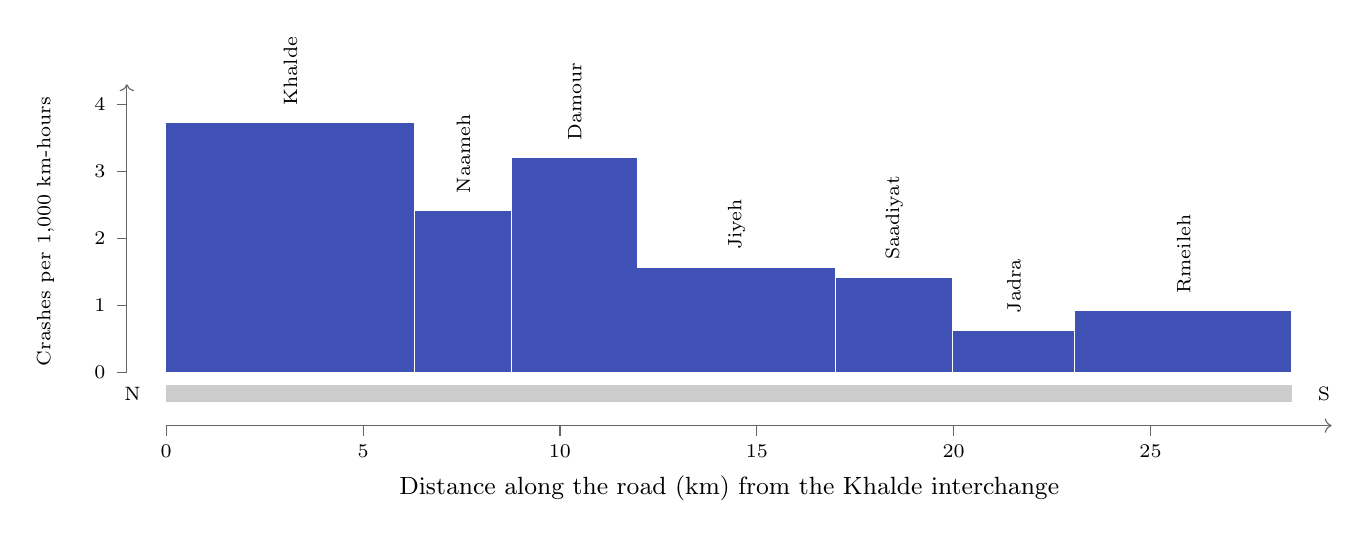
\begin{tikzpicture}[x=0.50cm,y=0.85cm,font=\small]
% --- y axis
\draw[->,black!60] (-1.0,0) -- (-1.0,4.3);
\foreach \yy in {0,1,2,3,4}{
  \draw[black!60] (-1.0,\yy) -- (-1.25,\yy);
  \node[left,font=\scriptsize] at (-1.3,\yy) {\yy};
}
\node[rotate=90,anchor=south,font=\scriptsize] at (-2.6,2.1)
  {Crashes per 1{,}000 km-hours};
% --- region bars: start / end / daytime rate / name
\foreach \xa/\xb/\hh/\nm in {%
  0/6.306/3.718/Khalde,
  6.306/8.786/2.408/Naameh,
  8.786/11.969/3.197/Damour,
  11.969/17.004/1.559/Jiyeh,
  17.004/19.982/1.411/Saadiyat,
  19.982/23.082/0.613/Jadra,
  23.082/28.6002/0.911/Rmeileh}
{
  \fill[barBlue] (\xa,0) rectangle (\xb,\hh);
  \draw[white,line width=0.7pt] (\xb,0) -- (\xb,\hh);
  \node[rotate=90,anchor=west,font=\scriptsize]
       at ({0.5*(\xa+\xb)},{\hh+0.12}) {\nm};
}
% --- road strip
\fill[black!20] (0,-0.45) rectangle (28.6002,-0.20);
\node[left,font=\scriptsize]  at (-0.4,-0.325) {N};
\node[right,font=\scriptsize] at (29.0,-0.325) {S};
% --- chainage axis
\draw[->,black!60] (0,-0.80) -- (29.6,-0.80);
\foreach \xx in {0,5,10,15,20,25}{
  \draw[black!60] (\xx,-0.80) -- (\xx,-0.95);
  \node[below,font=\scriptsize] at (\xx,-0.95) {\xx};
}
\node[below,font=\small] at (14.3,-1.40)
  {Distance along the road (km) from the Khalde interchange};
\end{tikzpicture}
\caption{The study road and its seven regions. The height of each bar is the
fitted daytime crash rate. The northern end, near Beirut, has about six times
the crash rate of the quietest southern region.}
\label{fig:corridor}
\end{figure}

\subsection{Data Sources}

The study rests on two main datasets, which come from two different
organisations. \textbf{The crash data come from the Lebanese Red Cross}: its
ambulance dispatch records give the date, time and town of every crash that an
ambulance attended. \textbf{The traffic data come from the National Council
for Scientific Research in Lebanon (CNRS-L)}: through a collaboration with
CNRS-L, we obtained a GPS dataset collected by the \emph{tari2ak} smartphone
application, which records the position and speed of phones in moving
vehicles. The Red Cross records tell us
how many crashes happened, and the CNRS-L GPS data tell us how busy and how fast
the road was at the same places and times. Three public sources complete the
picture: road geometry and landmarks from OpenStreetMap, hourly weather from
the ERA5 reanalysis, and a NOAA weather station used as a check.
Table~\ref{tab:sources} summarises all five.

\begin{table}[htbp]
\centering
\caption{Data sources and what each one provides. The first two rows are the
two main datasets.}
\label{tab:sources}
\small
\begin{tabular}{@{}lll@{}}
\toprule
\textbf{Source} & \textbf{Provides} & \textbf{Level of detail} \\
\midrule
Lebanese Red Cross ambulance dispatch records & Crash counts & Town name, date and time \\
CNRS-L GPS data (\emph{tari2ak} phone app) & Traffic level, speeds & Point, matched to the road \\
OpenStreetMap via Overpass~\cite{osm} & Road shape, ramps, landmarks & Every 100 m \\
Open-Meteo ERA5~\cite{hersbach2020} & Hourly weather & 3 points on the road \\
NOAA weather station 40100099999 & Weather check & Hourly, 1.7 km from km 0 \\
\bottomrule
\end{tabular}
\end{table}

The study period runs from 1 January 2016 to 31 July 2018, which is 31 full
months. We split each day into five time slots of different lengths: night
00--06 (6~h), morning rush 06--10 (4~h), daytime 10--16 (6~h), evening rush
16--20 (4~h) and late evening 20--24 (4~h).

\paragraph{Crash Data from the Lebanese Red Cross.}
\textbf{The ambulance records do not give exact locations.} The only location
in each record is the name of a town. Eight town names match places on the
study road. After merging one very small town with its neighbour, seven regions
remain. We fixed the borders between regions by placing known locations on the
road, which gives borders at 6.306, 8.786, 11.969, 17.004, 19.982 and
23.082~km. This level of detail comes from the records, not from our choice:
the road cannot be split into smaller parts, because the crash counts cannot be
split further.

Each record describes one patient, not one crash. Out of 24{,}628 patient
records, 1{,}807 are on the study road. We grouped them by region, date and
hour into \textbf{1{,}152 separate crashes}. We did not group them by exact
time, because the source files record seconds in 2016 but only minutes in later
years. Grouping by exact time would have dropped 32.5\% of the 2016 records,
against 5\% in later years, and would have shown a false 62\% rise in crashes
from one year to the next, against 9.5\% nationally. Table~\ref{tab:regions}
lists the crash count and the fixed features of each region.

\begin{table}[htbp]
\centering
\caption{The seven regions: position, length, crashes observed over the 31
months, and the features that stay the same across each region. RAF (roadside
activity factor) is the number of roadside landmarks per kilometre.}
\label{tab:regions}
\small
\begin{tabular}{@{}lrrrrrr@{}}
\toprule
\textbf{Region} & \textbf{Position (km)} & \textbf{Length (km)} & \textbf{Crashes} & \textbf{RAF} & \textbf{Curves ($^{\circ}$/km)} & \textbf{Ramps/mile} \\
\midrule
Khalde   & 0.000--6.306   & 6.306 & 437 & 4.123 & 37.2 & 2.79 \\
Naameh   & 6.306--8.786   & 2.480 & 140 & 2.419 & 49.6 & 4.32 \\
Damour   & 8.786--11.969  & 3.183 & 215 & 3.770 & 19.0 & 3.72 \\
Jiyeh    & 11.969--17.004 & 5.035 & 178 & 0.993 & 56.8 & 1.94 \\
Saadiyat & 17.004--19.982 & 2.978 &  81 & 1.007 & 37.1 & 1.61 \\
Jadra    & 19.982--23.082 & 3.100 &  26 & 0.000 & 50.3 & 1.26 \\
Rmeileh  & 23.082--28.600 & 5.518 &  75 & 0.725 & 55.7 & 4.84 \\
\midrule
Total    & 0.000--28.600  & 28.600 & 1{,}152 & & & \\
\bottomrule
\end{tabular}
\end{table}

\paragraph{Traffic Data from CNRS-L.}
Traffic is measured as a relative level, not an absolute count. Out of
6{,}006{,}401 GPS points in the CNRS-L dataset, 113{,}200 were within 150~m of
the road during the study period. The phone app that collected the points lost
users over these years, so raw counts would suggest a fall in traffic that
never happened. We therefore divided each count by the average for the whole
road in the same month. The traffic level $V$ shows only whether a place and
time is busier or quieter than average. The same GPS points give the speed
below which 85\% of drivers travel, $S85$. Cells with fewer than 30 GPS points
(22\% of cells) use the value for the same region and time slot instead.

\paragraph{Road Geometry and the Data Table.}
Road shape comes from 224 OpenStreetMap road pieces (3{,}387 points), which we
reduced to one centre line of 287 points by taking the middle of the two
carriageways every 50~m. Curvature is the total change of direction per
kilometre.

The table is built with every cell present, and cells with no crashes are kept
as zeros. \textbf{498 of the 1{,}085 cells (45.9\%) have no crashes}, and
these cells are essential: a model cannot estimate how often crashes happen
without also seeing the times and places where none happened.

\subsection{Methodological Framework}

Figure~\ref{fig:workflow} shows the full process, from the raw records to the
statistical model and on to the simulation and its results. The key point is
that the table of fitted rates is the only link between the model and the
simulator. It is the only thing the simulator knows about risk, and it is used
both to create crashes and to place the drones.

\begin{figure}[htbp]
\centering
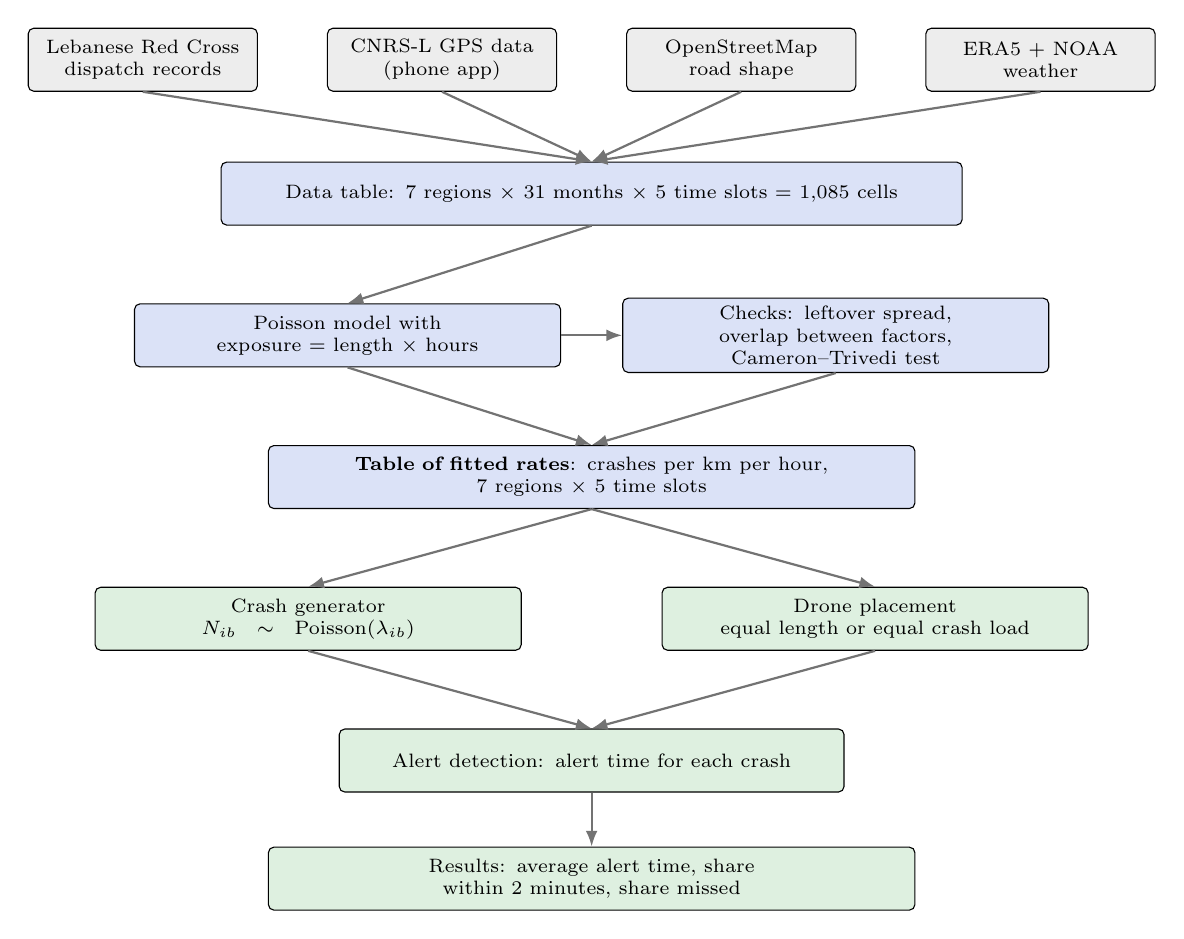
\begin{tikzpicture}[
  font=\scriptsize,
  bx/.style={draw,rounded corners=2pt,align=center,inner sep=3pt,
             minimum height=8mm},
  data/.style={bx,fill=boxData,text width=27mm},
  model/.style={bx,fill=boxModel},
  sim/.style={bx,fill=boxSim},
  ar/.style={-{Latex[length=2mm]},black!55,thick}]

\node[data] (d1) at (-5.7, 0)   {Lebanese Red Cross\\dispatch records};
\node[data] (d2) at (-1.9, 0)   {CNRS-L GPS data\\(phone app)};
\node[data] (d3) at ( 1.9, 0)   {OpenStreetMap\\road shape};
\node[data] (d4) at ( 5.7, 0)   {ERA5 + NOAA\\weather};

\node[model,text width=92mm] (panel) at (0,-1.7)
  {Data table: 7 regions $\times$ 31 months $\times$ 5 time slots
   = 1{,}085 cells};

\node[model,text width=52mm] (glm) at (-3.1,-3.5)
  {Poisson model with\\ exposure $=$ length $\times$ hours};
\node[model,text width=52mm] (diag) at ( 3.1,-3.5)
  {Checks: leftover spread,\\ overlap between factors, Cameron--Trivedi test};

\node[model,text width=80mm] (rate) at (0,-5.3)
  {\textbf{Table of fitted rates}: crashes per km per hour,\\
   7 regions $\times$ 5 time slots};

\node[sim,text width=52mm] (gen)   at (-3.6,-7.1)
  {Crash generator\\ $N_{ib}\sim\mathrm{Poisson}(\lambda_{ib})$};
\node[sim,text width=52mm] (alloc) at ( 3.6,-7.1)
  {Drone placement\\ equal length or equal crash load};

\node[sim,text width=62mm] (det) at (0,-8.9)
  {Alert detection: alert time for each crash};
\node[sim,text width=80mm] (met) at (0,-10.4)
  {Results: average alert time, share within 2 minutes, share missed};

\draw[ar] (d1.south) -- (panel.north);
\draw[ar] (d2.south) -- (panel.north);
\draw[ar] (d3.south) -- (panel.north);
\draw[ar] (d4.south) -- (panel.north);
\draw[ar] (panel.south) -- (glm.north);
\draw[ar] (glm.east)  -- (diag.west);
\draw[ar] (glm.south)  -- (rate.north);
\draw[ar] (diag.south) -- (rate.north);
\draw[ar] (rate.south) -- (gen.north);
\draw[ar] (rate.south) -- (alloc.north);
\draw[ar] (gen.south)   -- (det.north);
\draw[ar] (alloc.south) -- (det.north);
\draw[ar] (det.south) -- (met.north);
\end{tikzpicture}
\caption{The full process, from the data to the results. The crash counts come
from the Lebanese Red Cross and the traffic data from CNRS-L. The table of
fitted rates is the only way risk information reaches the simulator. It decides
both where crashes happen and where drones fly.}
\label{fig:workflow}
\end{figure}

\subsection{The Risk Model: What It Is and Why We Use It}

The whole system is built on one number:

\begin{quote}
$R$ = the expected number of crashes per kilometre of road per hour, for a
given stretch of the M51 at a given time of day.
\end{quote}

This is not a score. It has units, it was estimated from crashes that really
happened on this road, and it can be checked against the records. It has three
useful properties, and these are the reasons we chose it.

\begin{enumerate}[leftmargin=*,itemsep=2pt]
\item \emph{It can be added up over distance and time.} The expected number of
crashes on a stretch of length $\ell$ over $h$ hours is simply $R\,\ell\,h$. So
patrol segments of any length can be compared by the number of crashes they
are expected to see.
\item \emph{It predicts the yearly total instead of assuming it.} A score-based
system must be told how many crashes happen each year. A rate model predicts
this number. This means it can be wrong, and therefore it can be checked.
\item \emph{Time of day changes how many crashes happen, not only where.} With a
score, each time slot gets a fixed share of the day's crashes. With a rate, an
hour of rush-hour traffic can produce more crashes than an hour at night.
\end{enumerate}

\subsection{Model Specification}

Let $Y_{rmb}$ be the number of crashes in region $r$, month $m$ and time slot
$b$. The model is

\begin{equation}
Y_{rmb}\sim\mathrm{Poisson}(\mu_{rmb}),\qquad
\ln\mu_{rmb}=\ln E_{rmb}+\mathbf{x}_{rmb}'\boldsymbol{\beta},
\label{eq:glm}
\end{equation}

where $\mu_{rmb}$ is the expected number of crashes and the exposure is

\begin{equation}
E_{rmb}=L_r\times h_b\times d_m,
\label{eq:exposure}
\end{equation}

with $L_r$ the length of the region in kilometres, $h_b$ the length of the
time slot in hours, and $d_m$ the number of days in month $m$. The term
$\ln E_{rmb}$ is an \emph{offset}: it is added with a fixed weight of one, so
the rest of the model describes a rate per kilometre per hour instead of a raw
count. The risk factors enter as

\begin{equation}
\begin{aligned}
\mathbf{x}'\boldsymbol{\beta}=\ &\beta_0
+\beta_1\ln C_r
+\beta_2\ln(1+P_r)
+\beta_3\ln(1+\mathrm{RAF}_r)\\
&+\beta_4\ln V_{rb}
+\beta_5\ln S85_{rb}
+\beta_6\sin\!\Big(\tfrac{2\pi m}{12}\Big)
+\beta_7\cos\!\Big(\tfrac{2\pi m}{12}\Big),
\end{aligned}
\label{eq:linpred}
\end{equation}

where $C_r$ is how curved the road is (degrees per kilometre), $P_r$ is the
number of ramps per mile, $\mathrm{RAF}_r$ is the number of roadside landmarks
per kilometre, $V_{rb}$ is the relative traffic level from the CNRS-L GPS
data, and $S85_{rb}$ is the speed below which 85\% of drivers travel, from the
same data. The sine and cosine terms describe a smooth yearly cycle. We use
the logarithm of each factor, so $\exp(\beta_j)$ is a \emph{rate ratio}: the
number by which the crash rate is multiplied when the logarithm of that factor
goes up by one. Factors that can be zero use $\ln(1+x)$.

We make four assumptions clear. (A1) Once the risk factors and the exposure are
known, the crash counts in different cells do not depend on each other. (A2)
Crashes rise in proportion to exposure. (A3) Region features are the same
everywhere inside a region, so for these features there are only seven
independent values, not 1{,}085. (A4) Each crash belongs to the region of the
town that reported it.

\paragraph{Choosing between Poisson and Negative Binomial.}
We fitted both a Poisson model and a negative binomial model, and we fixed the
rule for choosing between them in advance. We would use the negative binomial
if the leftover spread after fitting (the Pearson residual dispersion) was
above 1.25, or if the Cameron--Trivedi test was significant with a positive
slope, or if the negative binomial improved AIC by more than 4. (AIC is a score
for how well a model fits, with a penalty for extra terms; lower is better.)
Otherwise we would keep the Poisson model.

Before fitting, the raw crash counts vary 1.744 times as much as their average,
which would usually suggest overdispersion. After fitting, however, the
leftover spread is only 1.13, the Cameron--Trivedi slope is 0.058 ($t=1.43$,
$p=0.152$, not significant), and the negative binomial improves AIC by only
3.4. \textbf{We therefore keep the Poisson model.} The extra variation in the
raw counts is explained by the risk factors and the exposure~\cite{cameron1990}.

\paragraph{Terms We Tested and Dropped.}
We also tried other risk factors and model forms, and dropped them.
Table~\ref{tab:rejected} lists them with the reason, so that the reader can see
what the final model does not include.

\begin{table}[htbp]
\centering
\caption{Model terms we tested and dropped.}
\label{tab:rejected}
\small
\begin{tabular}{@{}p{4.1cm}p{10.6cm}@{}}
\toprule
\textbf{Tested} & \textbf{Why it was dropped} \\
\midrule
Weather (share of wet hours) & It only mattered when there was no seasonal
term, because it simply followed the calendar (0.288 of hours wet in January,
0.008 in August). With the seasonal terms included, its rate ratio was 1.008,
meaning no effect. \\
Roadside activity weighted by distance & It needed four settings that could not
be measured on this road, and 40 of the 56 landmarks had no review data. The
simple landmark count did better in 7 of 8 tests where one region was left out. \\
Roadside activity by time slot & It fell to almost zero at night, just like
traffic. It repeated the time-of-day pattern that traffic already carries, and
made the traffic term change sign. \\
Traffic inside the exposure term & The traffic factor became redundant, and its
coefficient flipped from $+0.236$ to $-0.847$. \\
One combined road-shape factor & Curves and ramps act in opposite directions on
this road, so a single combined factor only showed their average. We split it
into two terms. \\
Negative binomial model & The leftover spread was only 1.13, the
Cameron--Trivedi test was not significant, and the AIC improved by only 3.4. \\
\bottomrule
\end{tabular}
\end{table}

\subsection{From Coefficients to a Rate Table}

The model gives one prediction per cell. The simulator needs one rate per
region and time slot, so we add up the predictions over all months and divide
by the total exposure:

\begin{equation}
R_{rb}=\frac{\sum_m \hat{\mu}_{rmb}}{\sum_m E_{rmb}}
\qquad[\text{crashes per km per hour}].
\label{eq:aggregate}
\end{equation}

Because we average over whole years, the yearly cycle cancels out, so $R_{rb}$
is an average for the whole year.

The simulator divides the road into 1~km sections, which gives 29 sections. The
region borders do not fall on whole kilometres, so six of the 29 sections lie
across two regions. The rate of such a section is the average of the two
regions' rates, weighted by how much of the section lies in each:

\begin{equation}
R_{ib}=\frac{\sum_r R_{rb}\,\lambda(i\cap r)}{\sum_r \lambda(i\cap r)},
\label{eq:blend}
\end{equation}

where $\lambda(i\cap r)$ is the length of section $i$ that lies in region $r$.
This detail matters. If each section were simply given to the region at its
midpoint, 0.8\% of all crashes would be lost, and the total check in
Section~\ref{sec:validation} would fail.

\subsection{Generating Crashes}

For each section $i$, each time slot $b$ and each simulated day,

\begin{equation}
\lambda_{ib}=R_{ib}\,\ell_i\,h_b,\qquad
N_{ib}\sim\mathrm{Poisson}(\lambda_{ib}),\qquad
\tau\sim U(\text{slot start},\ \text{slot end}),\qquad
s\sim U(s_i^{\text{start}},\ s_i^{\text{end}}).
\label{eq:generate}
\end{equation}

In words: the expected number of crashes $\lambda_{ib}$ is the rate times the
section length $\ell_i$ times the slot length $h_b$; the actual number
$N_{ib}$ is drawn at random around this value; and each crash is given a random
time $\tau$ inside the slot and a random position $s$ inside the section. Every
section and slot is drawn on its own. The simulator is never told the yearly
total. It simply comes out of the rates.

\subsection{The UAV Swarm and Its Allocation}

The swarm has $M$ identical drones. Each drone is given one patrol segment
$[A_j,B_j]$ of the road and flies back and forth along it at a constant speed
$v$. We compare two ways of building the segments.

\paragraph{Uniform.}
The road of length $L$ is cut into $M$ equal pieces, with $A_j=(j-1)L/M$ and
$B_j=jL/M$. This plan uses no risk information. It is the baseline.

\paragraph{Risk-aware.}
The 1~km sections are grouped so that each drone has about the same expected
number of crashes. The daily crash load of section $i$ is
$\rho_i=\sum_b\lambda_{ib}$, and the target for each drone is
$\bar{\rho}=\sum_i\rho_i/M$. Starting from the northern end, sections are added
to a segment until its load reaches the target. The section at the border goes
to whichever side ends up closer to the target, and the last segment takes
whatever is left. When there are more drones than sections, the extra drones
are shared among the busiest segments using Hamilton's largest-remainder
method~\cite{balinski1982}. Drones that share a segment start at evenly spaced
points and fly in opposite directions, so that they do not fly side by side.

Equal crash load is not the same as equal length.
Figure~\ref{fig:partition} shows the two plans with five drones.

\begin{figure}[htbp]
\centering
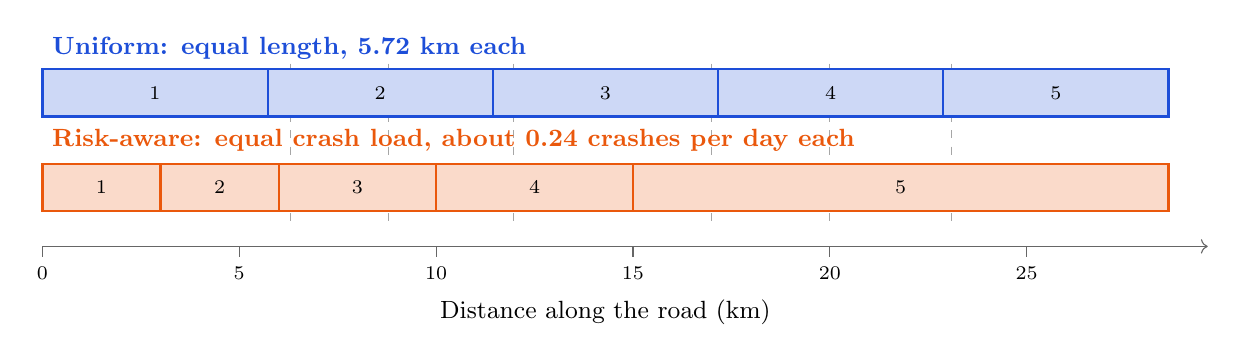
\begin{tikzpicture}[x=0.50cm,y=1.0cm,font=\small]
% --- region borders (drawn first, behind the boxes)
\foreach \xx in {6.306,8.786,11.969,17.004,19.982,23.082}
  \draw[black!35,dashed] (\xx,1.22) -- (\xx,-0.88);
% --- uniform row
\node[anchor=west,font=\small\bfseries,text=polUniform] at (0,1.42)
  {Uniform: equal length, 5.72 km each};
\foreach \xa/\xb/\nm in {0/5.72/1, 5.72/11.44/2, 11.44/17.16/3,
                         17.16/22.88/4, 22.88/28.6002/5}{
  \fill[polUniform!22] (\xa,0.55) rectangle (\xb,1.15);
  \draw[polUniform,thick]  (\xa,0.55) rectangle (\xb,1.15);
  \node[font=\scriptsize] at ({0.5*(\xa+\xb)},0.85) {\nm};
}
% --- risk-aware row
\node[anchor=west,font=\small\bfseries,text=polRisk] at (0,0.25)
  {Risk-aware: equal crash load, about 0.24 crashes per day each};
\foreach \xa/\xb/\nm in {0/3/1, 3/6/2, 6/10/3, 10/15/4, 15/28.6002/5}{
  \fill[polRisk!22] (\xa,-0.65) rectangle (\xb,-0.05);
  \draw[polRisk,thick] (\xa,-0.65) rectangle (\xb,-0.05);
  \node[font=\scriptsize] at ({0.5*(\xa+\xb)},-0.35) {\nm};
}
% --- distance axis
\draw[->,black!60] (0,-1.10) -- (29.6,-1.10);
\foreach \xx in {0,5,10,15,20,25}{
  \draw[black!60] (\xx,-1.10) -- (\xx,-1.24);
  \node[below,font=\scriptsize] at (\xx,-1.24) {\xx};
}
\node[below,font=\small] at (14.3,-1.65) {Distance along the road (km)};
\end{tikzpicture}
\caption{The two patrol plans with five drones. Dashed lines are region
borders, and each numbered box is one drone's patrol segment. The uniform plan
gives every drone 5.72~km. The risk-aware plan gives every drone about the same
number of expected crashes, so two drones share the first 6~km and one drone
covers the last 13.6~km.}
\label{fig:partition}
\end{figure}

\subsection{Detection through the IoT Alert}
\label{sec:detection}

Detection is modelled as a radio signal, not a camera image. The IoT sensors
are mounted on the guardrail, the metal crash barrier that runs along the side
of the road, so they sit right next to the traffic and need no extra poles or
roadworks. When a crash happens at position $s_k$, the guardrail sensor at
that point sends an alert. Any drone inside the \emph{alert zone}
$[s_k-R_{\mathrm{IoT}},\,s_k+R_{\mathrm{IoT}}]$ receives it at once. The drones
do not change course when a crash happens: the alert time is simply how long
their normal patrol takes to bring one of them into the alert zone.

A drone that patrols $[A_j,B_j]$, a segment of length $L_j$, has position $s_j$
and direction $d_j$ ($+1$ when flying south, $-1$ when flying north):

\begin{equation}
q_j(t)=(v\,t)\bmod 2L_j,\qquad
s_j=\begin{cases} A_j+q_j, & q_j\le L_j,\\ B_j-(q_j-L_j), & \text{otherwise,}\end{cases}
\qquad
d_j=\begin{cases}+1, & q_j\le L_j,\\ -1, & \text{otherwise.}\end{cases}
\label{eq:motion}
\end{equation}

The part of the alert zone that the drone can reach is where the zone overlaps
its segment:

\begin{equation}
O_j=\big[\max(A_j,\ s_k-R_{\mathrm{IoT}}),\ \min(B_j,\ s_k+R_{\mathrm{IoT}})\big]
=[O^-,\,O^+].
\label{eq:overlap}
\end{equation}

If there is no overlap, this drone can never receive the alert. Otherwise, the
time until the drone first enters the zone is

\begin{equation}
T_j=
\begin{cases}
0, & s_j\in[O^-,O^+],\\[2pt]
(O^--s_j)/v, & s_j<O^-,\ d_j=+1,\\[2pt]
\big[(s_j-A_j)+(O^--A_j)\big]/v, & s_j<O^-,\ d_j=-1,\\[2pt]
(s_j-O^+)/v, & s_j>O^+,\ d_j=-1,\\[2pt]
\big[(B_j-s_j)+(B_j-O^+)\big]/v, & s_j>O^+,\ d_j=+1.
\end{cases}
\label{eq:cases}
\end{equation}

In words: in the first case the drone is already in range. In the second and
fourth cases it is flying towards the zone, so the time is the distance divided
by the speed. In the third and fifth cases it is flying away, so it must first
reach the end of its segment, turn around, and come back.

Only three segments can reach the crash first: the segment $m$ that contains
the crash and its two neighbours. The alert time for crash $k$ is therefore the
shortest time among the drones in these segments:

\begin{equation}
T_{\mathrm{alert},k}=\min_{j\in\{m-1,\,m,\,m+1\}}\ \ \min_{\text{drones in }j}\ T_j .
\label{eq:talert}
\end{equation}

A crash is counted as \emph{missed} if no drone can reach its zone, or if the
alert time is longer than the 600~s detection window.

We set the alert range to 200~m on purpose, well below what the radio can
reach. Field tests show that LoRa radios can reach several
kilometres~\cite{petajajarvi2015}. At such ranges the alert zone covers most of
the road, the nearest drone almost always hears the alert at once, and the
choice of patrol plan stops mattering. At 200~m, where the drones fly is what
limits detection, so the two plans can be compared.
Section~\ref{sec:sensitivity} shows what happens at longer ranges.

We also built a small hardware prototype of this alert chain. A tilt sensor
node (an ESP32 board with an MPU6050 motion sensor), designed to be fixed to
the roadside guardrail, detects the sudden movement of the barrier and sends an
alert over ESP-NOW to a drone hub, which passes it on over a 433~MHz LoRa radio
(Ai-Thinker Ra-02) to a home base. The home base stores each event in an online
database, and the planning application shows the events on a live page. The
prototype shows that the alert chain can be built, but this paper reports no
measurements from it.

\subsection{Operational Layer}

Real drones cannot fly forever, so the simulator includes batteries. A
patrolling drone uses 2\% of its battery per minute, which gives about 50
minutes of flight. When the battery drops below 25\%, the drone leaves its
segment, flies to a dock (60~s), recharges, and returns once it is above 80\%.
While it is away, its segment has no drone unless a spare drone takes its
place. A pool of $\max(2,\lceil M/8\rceil)$ spare drones fills these gaps after
a 30~s delay. These rules decide whether a fleet of $M$ drones really has $M$
drones in the air. At the start of each trial, every drone begins at a random
point of its segment, in a random direction, with a battery level between 60\%
and 100\%.

\subsection{Experimental Design and Metrics}

Table~\ref{tab:params} lists the simulation settings. Each trial covers 30
simulated days in steps of 5~s, at the road's real fitted crash rate. We did
not increase the crash rate to get more events. We tested fleets of
$M\in\{1,2,3,5,7,10,13,16,20,25,30\}$ drones, with 50 trials for each fleet
size and each plan. This gives about 1{,}800 crashes behind every point in the
results. For each trial and fleet size, both plans face \emph{exactly the same}
crashes, because crashes are created by their own random number generator,
separate from the one used to place the drones. The runs can be repeated
exactly: the random seed for trial $t$ is $42+1009\,t+7919\,M$.

We report three results. The \emph{average alert time} is the mean time to
detection over the crashes that were detected. The \emph{two-minute share},
$P(T\le 120\,\mathrm{s})$, is the share of \emph{all} crashes detected within
two minutes, so missed crashes count against it. The \emph{missed share} is
the share of crashes not detected within the 600~s window.

\begin{table}[htbp]
\centering
\caption{Simulation settings.}
\label{tab:params}
\small
\begin{tabular}{@{}llll@{}}
\toprule
\textbf{Setting} & \textbf{Value} & \textbf{Setting} & \textbf{Value} \\
\midrule
Time step $\Delta t$        & 5 s     & Battery use              & 2\%/min \\
Trial length                & 30 days & Return-to-dock level     & 25\% \\
Trials per point            & 50      & Ready-to-fly level       & 80\% \\
Drone speed $v$             & 8 m/s   & Flight to dock           & 60 s \\
Alert range $R_{\mathrm{IoT}}$ & 200 m & Charging               & 0 to 100\% in 240 s \\
Detection window            & 600 s   & Spare drones             & $\max(2,\lceil M/8\rceil)$ \\
Section size                & 1 km (29 sections) & Spare drone delay & 30 s \\
Trial start time            & 08:00   & Crash rate               & fitted, not increased \\
\bottomrule
\end{tabular}
\end{table}

\subsection{Implementation}
\label{sec:impl}

The model was fitted in Python with statsmodels~\cite{seabold2010}. An export
script, kept with the data panel and not part of the public repository, refits
the model and writes the rate table to one file
(\texttt{risk-table.json}), together with the formula, the coefficients and the
leftover spread, so that every rate can be traced back to the fit. The script
stops with an error if the yearly total from the table differs from the
observed total by more than one crash.

The simulator is part of a web application, the Simulation-Aided Command
Center, written in JavaScript with React, and it runs fully in the web
browser. It uses a seeded random number generator (mulberry32) and draws
Poisson counts with Knuth's method~\cite{knuth1997}. The source code is openly
available on GitHub~\cite{thesiscode}, and a live version of the application
can be used in any web browser~\cite{thesisapp}. The model and simulation code
has about 3{,}200 lines in ten JavaScript files, in the
\texttt{src/partitioning/lib} and \texttt{src/detection/lib} folders.
Table~\ref{tab:codemap} shows where each part described in this paper is
implemented. For this paper, we ran the
same code outside the browser with Node.js 24.18.1, without changing the
simulation code. The project has no automated tests; the checks in
Section~\ref{sec:validation} were run as scripts that use the application's own
code.

\begin{table}[htbp]
\centering
\caption{Where each part of the system is implemented. All files are in the
\texttt{src} folder of the project repository~\cite{thesiscode}.}
\label{tab:codemap}
\small
\begin{tabular}{@{}p{4.2cm}p{4.3cm}p{6.2cm}@{}}
\toprule
\textbf{Part} & \textbf{File} & \textbf{Main functions} \\
\midrule
Fitted rates and their source & \texttt{risk-table.json} & (data file) \\
Region lookup and blending & \texttt{risk-scoring.js} & \texttt{rateOverSpan}, \texttt{buildRiskMatrix} \\
Crash generation & \texttt{accident-generator.js} & \texttt{samplePoisson}, \texttt{generateAccidentsForDay} \\
Patrol segments & \texttt{uav-segments.js} & \texttt{buildUniformSegments}, \texttt{buildRiskAwareSegments} \\
Drone motion and alert time & \texttt{iot-alert.js} & \texttt{patrolPositionAndDirection}, \texttt{alertTimeForCandidateAtState}, \texttt{computeIotDetection} \\
Trial loop, batteries, spare drones & \texttt{detection-sim.js} & \texttt{simulateOnce}, \texttt{DEFAULT\_PARAMS}, \texttt{makeRng} \\
Repeated trials & \texttt{monteCarlo.js} & \texttt{runSweep} \\
\bottomrule
\end{tabular}
\end{table}

% ===========================================================================
\section{Results}

\subsection{The Fitted Rate Surface}

Table~\ref{tab:coef} shows the fitted model. All five risk factors and both
seasonal terms are significant at the 5\% level.

\begin{table}[htbp]
\centering
\caption{The fitted Poisson model with exposure offset. $n=1{,}085$ cells;
AIC $=2648.9$; leftover spread (residual dispersion) $=1.13$. The rate ratio is
$\exp(\beta)$.}
\label{tab:coef}
\small
\begin{tabular}{@{}lrrlr@{}}
\toprule
\textbf{Term} & $\hat{\beta}$ & \textbf{SE} & \textbf{Rate ratio [95\% CI]} & $p$ \\
\midrule
Intercept                 & $-21.923$ & 3.442 & ---                        & $<0.001$ \\
$\ln$ curvature           & $+0.225$  & 0.111 & 1.25 [1.01, 1.56]          & 0.043 \\
$\ln(1+$ramp density$)$   & $-0.361$  & 0.128 & 0.70 [0.54, 0.90]          & 0.005 \\
$\ln(1+$RAF$)$            & $+1.344$  & 0.104 & \textbf{3.84 [3.13, 4.70]} & $<0.001$ \\
$\ln$ traffic level       & $+0.388$  & 0.054 & 1.47 [1.33, 1.64]          & $<0.001$ \\
$\ln$ speed ($S85$)       & $+3.010$  & 0.700 & 20.29 [5.14, 80.02]        & $<0.001$ \\
Season (sine)             & $-0.108$  & 0.043 & 0.90 [0.83, 0.98]          & 0.012 \\
Season (cosine)           & $-0.125$  & 0.042 & 0.88 [0.81, 0.96]          & 0.003 \\
\bottomrule
\end{tabular}
\end{table}

\paragraph{Roadside Activity Matters Most.}
If $(1+\mathrm{RAF})$ doubles, the crash rate is multiplied by 2.54. This
factor is also estimated much more precisely than any other ($z=12.97$). We
also added the factors to the model one at a time and recorded how much each
one improved the fit (Figure~\ref{fig:aic}). Roadside activity improved AIC by
192.0, more than twice as much as the next factor, curvature (91.8). Traffic
added 36.3, speed 16.6 and ramps 5.3. On a road with poorly controlled access,
what happens beside the road matters more than the shape of the road.

\begin{figure}[htbp]
\centering
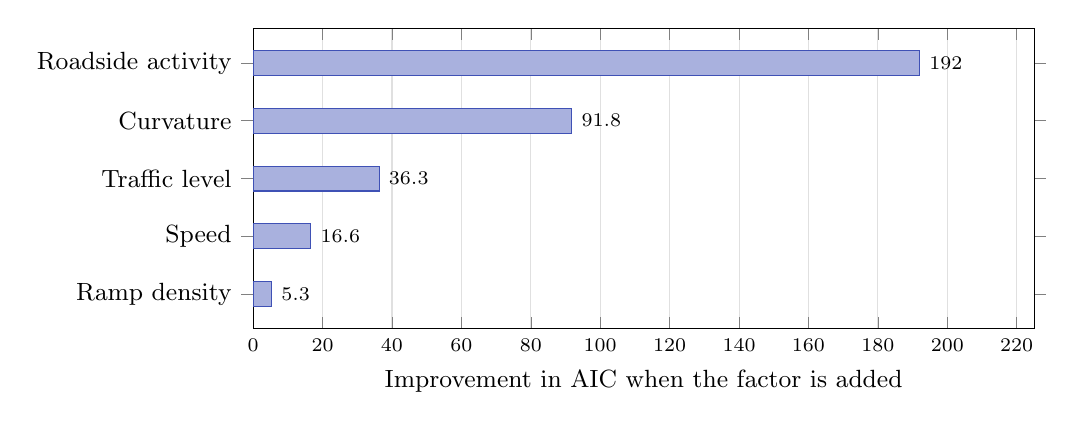
\begin{tikzpicture}
\begin{axis}[
  xbar, width=11.5cm, height=5.4cm,
  xmin=0, xmax=225,
  bar width=9pt,
  symbolic y coords={Ramp density,Speed,Traffic level,Curvature,Roadside activity},
  ytick=data,
  yticklabel style={font=\small},
  xticklabel style={font=\scriptsize},
  xlabel={Improvement in AIC when the factor is added},
  xlabel style={font=\small},
  xmajorgrids, grid style={black!12},
  nodes near coords, point meta=x,
  nodes near coords style={font=\scriptsize,anchor=west},
  enlarge y limits=0.15]
\addplot[draw=barBlue,fill=barBlue!45] coordinates
 {(5.3,Ramp density)(16.6,Speed)(36.3,Traffic level)(91.8,Curvature)(192.0,Roadside activity)};
\end{axis}
\end{tikzpicture}
\caption{How much each factor improves the model when it is added. A bigger
improvement means the factor explains more of the crash pattern. Roadside
activity adds more than twice as much as any other factor.}
\label{fig:aic}
\end{figure}

\paragraph{More Ramps, Fewer Crashes.}
Regions with more ramps have fewer crashes per kilometre-hour (rate ratio 0.70,
$p=0.005$). This is the opposite of what most studies find~\cite{park2010}. We
report it as a pattern in the data, not as a cause, and
Section~\ref{sec:discussion} explains why. This factor only acts inside the
fitted rates; the simulator never uses it on its own, so nothing in the system
claims that ramps make a road safer.

\paragraph{The Factors Do Not Overlap Too Much.}
The variance inflation factors, which measure how much the risk factors overlap
with each other, range from 1.53 to 3.16. All are well below the usual warning
levels.

Applying Equation~\ref{eq:aggregate} gives the table of rates in
Table~\ref{tab:rates}, shown as a chart in Figure~\ref{fig:rates}. Two patterns
stand out. The rate falls steadily from north to south. And in every region,
the daytime rate is 1.4 to 2.0 times the night rate.

\begin{table}[htbp]
\centering
\caption{Fitted crash rates, in crashes per 1{,}000 kilometre-hours, by region
and time slot. Regions are sorted by their daytime rate.}
\label{tab:rates}
\small
\begin{tabular}{@{}lrrrrrr@{}}
\toprule
\textbf{Region} & \textbf{Night} & \textbf{Morning} & \textbf{Daytime} & \textbf{Evening} & \textbf{Late} & \textbf{Day/night} \\
       & 00--06 & 06--10 & 10--16 & 16--20 & 20--24 & \textbf{ratio} \\
\midrule
Khalde   & 2.412 & 3.536 & 3.718 & 3.631 & 3.379 & 1.54 \\
Damour   & 1.951 & 3.098 & 3.197 & 3.289 & 2.846 & 1.64 \\
Naameh   & 1.683 & 2.227 & 2.408 & 2.312 & 2.150 & 1.43 \\
Jiyeh    & 0.815 & 1.514 & 1.559 & 1.532 & 1.254 & 1.91 \\
Saadiyat & 0.827 & 1.364 & 1.411 & 1.366 & 1.084 & 1.71 \\
Rmeileh  & 0.463 & 0.869 & 0.911 & 0.864 & 0.636 & 1.97 \\
Jadra    & 0.366 & 0.609 & 0.613 & 0.579 & 0.491 & 1.68 \\
\bottomrule
\end{tabular}
\end{table}

\begin{figure}[htbp]
\centering
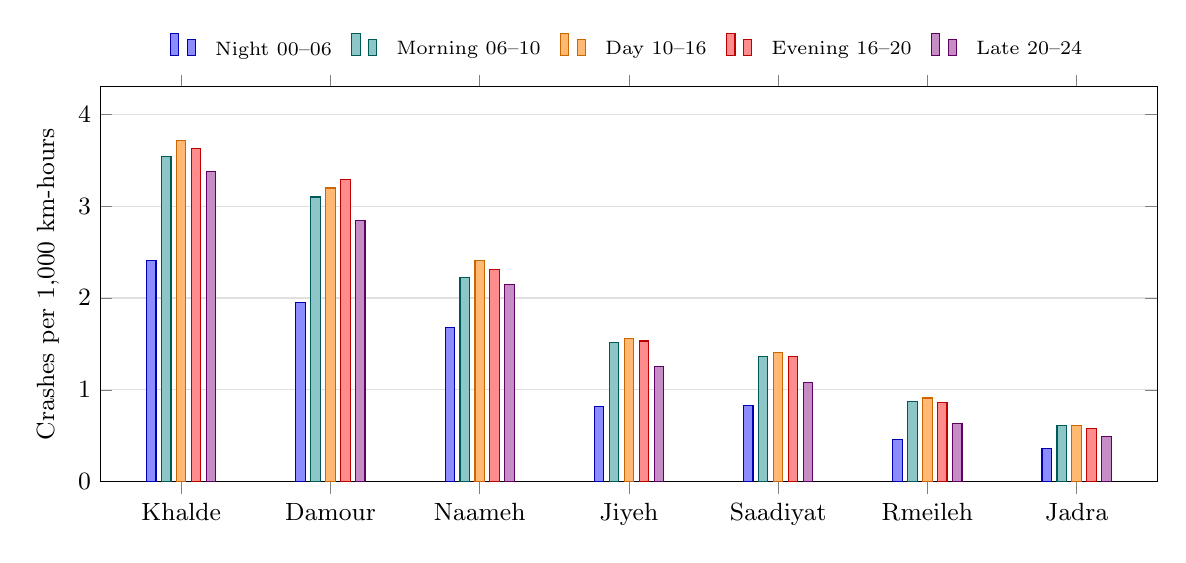
\begin{tikzpicture}
\begin{axis}[
  width=15cm, height=6.6cm,
  ybar, bar width=3.4pt,
  ymin=0, ymax=4.3,
  ylabel={Crashes per 1{,}000 km-hours},
  ylabel style={font=\small},
  symbolic x coords={Khalde,Damour,Naameh,Jiyeh,Saadiyat,Rmeileh,Jadra},
  xtick=data,
  xticklabel style={font=\small},
  yticklabel style={font=\small},
  ymajorgrids, grid style={black!12},
  legend style={at={(0.5,1.04)},anchor=south,legend columns=5,
                draw=none,font=\scriptsize,column sep=5pt},
  enlarge x limits=0.09]
\addplot[draw=blue!70!black,fill=blue!45] coordinates
 {(Khalde,2.412)(Damour,1.951)(Naameh,1.683)(Jiyeh,0.815)
  (Saadiyat,0.827)(Rmeileh,0.463)(Jadra,0.366)};
\addplot[draw=teal!70!black,fill=teal!45] coordinates
 {(Khalde,3.536)(Damour,3.098)(Naameh,2.227)(Jiyeh,1.514)
  (Saadiyat,1.364)(Rmeileh,0.869)(Jadra,0.609)};
\addplot[draw=orange!80!black,fill=orange!55] coordinates
 {(Khalde,3.718)(Damour,3.197)(Naameh,2.408)(Jiyeh,1.559)
  (Saadiyat,1.411)(Rmeileh,0.911)(Jadra,0.613)};
\addplot[draw=red!75!black,fill=red!45] coordinates
 {(Khalde,3.631)(Damour,3.289)(Naameh,2.312)(Jiyeh,1.532)
  (Saadiyat,1.366)(Rmeileh,0.864)(Jadra,0.579)};
\addplot[draw=violet!75!black,fill=violet!45] coordinates
 {(Khalde,3.379)(Damour,2.846)(Naameh,2.150)(Jiyeh,1.254)
  (Saadiyat,1.084)(Rmeileh,0.636)(Jadra,0.491)};
\legend{Night 00--06, Morning 06--10, Day 10--16, Evening 16--20, Late 20--24}
\end{axis}
\end{tikzpicture}
\caption{Fitted crash rate by region and time slot. The order of the regions is
the same in every time slot, and night is always the lowest. Khalde has about
six times the rate of Jadra.}
\label{fig:rates}
\end{figure}

\subsection{Validation}
\label{sec:validation}

A big advantage of a rate model over a score is that it can be checked against
the records. We ran three checks.

\paragraph{Total for the Whole Road.}
Adding up $R_{ib}\,\ell_i\,h_b$ over all 29 sections, all five time slots and
365 days gives \textbf{445.9 crashes per year}. This is the same as the 1{,}152
crashes observed in 31 months. This match is expected: in a Poisson model with
a log link and an intercept, the predicted values always add up to the observed
total~\cite{mccullagh1989}. So this check does not prove that the model is
right. What it does show is that no crashes were lost when we turned the model
into a rate table and spread it over the 1~km sections. This is how we found
that the midpoint method lost 0.8\% of crashes.

\paragraph{Totals by Region.}
The model has no separate term for each region, so nothing forces the regional
totals to match. This makes it a real test. Figure~\ref{fig:validation}
compares predicted and observed crashes for each region over the 31 months. The
correlation is 0.990. Khalde is slightly over-predicted (469 against 437 observed)
and Jiyeh under-predicted (149 against 178). The largest relative error is in
Jadra, the region with the fewest crashes, where 37 crashes are predicted
against 26 observed.

\paragraph{Totals by Time of Day.}
One weakness should be reported. The model predicts too many crashes in the
morning rush (211 predicted, 136 observed) and too few in the evening rush (217
predicted, 279 observed). Traffic and speed are similar in the two rush hours,
so the model cannot tell them apart, even though the real counts differ by a
factor of two. Section~\ref{sec:discussion} returns to this.

All three checks use the same data that the model was fitted on. No crashes
were kept aside for testing.

\paragraph{Checks on the Simulator.}
We also checked that the simulator produces what the rates say. Across the 550
trials of one plan in our experiment, it created 20{,}241 crashes: 36.80 per
30-day trial, or 447.8 per year, against 445.9 expected. The difference is
0.4\%, well within random variation. Running the same trial twice with the same
seed gave exactly the same crashes and alert times, and both plans saw exactly
the same crashes.

\begin{figure}[htbp]
\centering
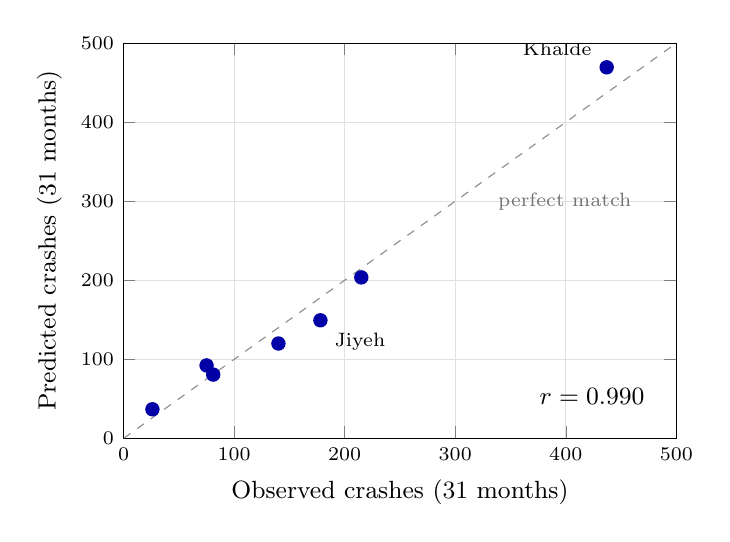
\begin{tikzpicture}
\begin{axis}[
  width=8.6cm, height=6.6cm,
  xlabel={Observed crashes (31 months)},
  ylabel={Predicted crashes (31 months)},
  xlabel style={font=\small}, ylabel style={font=\small},
  xmin=0,xmax=500,ymin=0,ymax=500,
  xtick={0,100,200,300,400,500}, ytick={0,100,200,300,400,500},
  ticklabel style={font=\scriptsize},
  grid=both, grid style={black!12}]
\addplot[dashed,black!45,domain=0:500,forget plot] {x};
\addplot[only marks,mark=*,mark size=2.4pt,color=blue!65!black,forget plot]
 coordinates {(437,469.4)(140,119.9)(215,203.6)(178,149.3)
              (81,80.6)(26,36.7)(75,92.2)};
\node[font=\small,anchor=south east] at (axis cs:480,30) {$r=0.990$};
\node[font=\scriptsize,anchor=west,text=black!55] at (axis cs:330,300) {perfect match};
\node[font=\scriptsize,anchor=south east] at (axis cs:432,472) {Khalde};
\node[font=\scriptsize,anchor=north west] at (axis cs:182,146) {Jiyeh};
\end{axis}
\end{tikzpicture}
\caption{Observed against predicted crashes for each region over the 31 months.
Each dot is one region, and the dashed line shows a perfect match. The regions
agree closely. For single cells the correlation drops to 0.609, which is
expected, because 45.9\% of cells have no crashes and no cell has more than
seven.}
\label{fig:validation}
\end{figure}

\subsection{What the Two Policies Do to the Corridor}

Because risk is now measured in crashes per day, we can read each patrol
segment directly. With five drones, the target is about 0.24 expected crashes
per day for each drone. Table~\ref{tab:segments} shows the result, which is
drawn in Figure~\ref{fig:partition}.

\begin{table}[htbp]
\centering
\caption{Risk-aware patrol segments with five drones. Each drone has about the
same number of expected crashes, but the longest segment is 4.5 times as long
as the shortest.}
\label{tab:segments}
\small
\begin{tabular}{@{}crrrl@{}}
\toprule
\textbf{Drone} & \textbf{Segment (km)} & \textbf{Length (km)} & \textbf{Expected crashes per day} & \textbf{Regions covered} \\
\midrule
1 & 0.0--3.0   & 3.0  & 0.237 & Khalde \\
2 & 3.0--6.0   & 3.0  & 0.237 & Khalde \\
3 & 6.0--10.0  & 4.0  & 0.234 & Khalde, Naameh, Damour \\
4 & 10.0--15.0 & 5.0  & 0.229 & Damour, Jiyeh \\
5 & 15.0--28.6 & 13.6 & 0.285 & Jiyeh, Saadiyat, Jadra, Rmeileh \\
\midrule
\multicolumn{5}{@{}l@{}}{\emph{Uniform plan, for comparison:} five segments of 5.72~km each.}\\
\bottomrule
\end{tabular}
\end{table}

Two drones now share the first 6~km, while one drone covers the last 13.6~km.
This is what the plan is meant to do: more drones where there are more crashes.
It is also the opposite of what the earlier expert-score version did. That
version gave the highest traffic score to \emph{both} ends of the road, and so
placed many drones in the south. The crash records show that the southern end
is actually the quietest part of the road.

\subsection{Detection Performance against Fleet Size}

Figure~\ref{fig:perf} shows the two main results, and Table~\ref{tab:sweep}
gives the numbers behind them.

\begin{figure}[htbp]
\centering
\begin{minipage}[t]{0.48\textwidth}
\centering
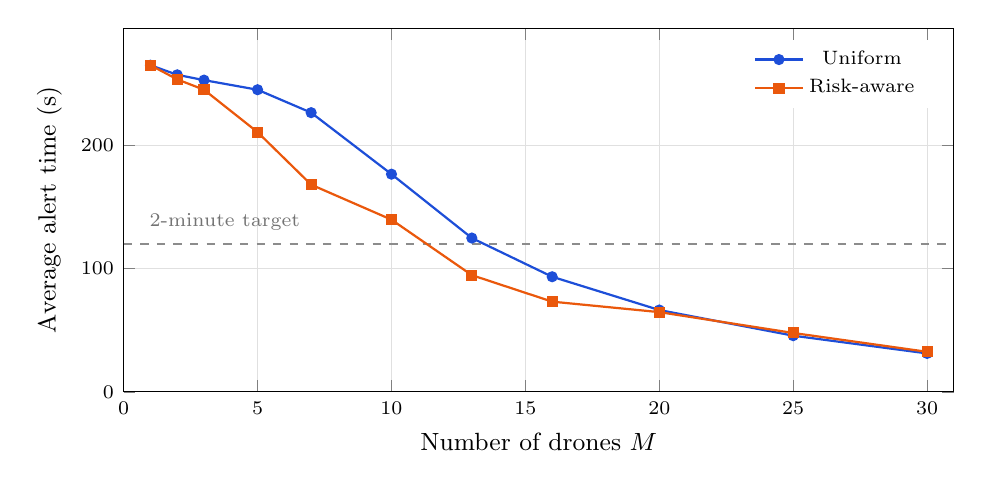
\begin{tikzpicture}
\begin{axis}[
  width=\linewidth, height=6.2cm,
  xlabel={Number of drones $M$}, ylabel={Average alert time (s)},
  xlabel style={font=\small}, ylabel style={font=\small},
  ticklabel style={font=\scriptsize},
  xmin=0,xmax=31,ymin=0,ymax=295,
  grid=both, grid style={black!12},
  legend style={at={(0.97,0.97)},anchor=north east,draw=none,font=\scriptsize}]
\addplot[dashed,black!45,domain=0:31,forget plot] {120};
\node[font=\scriptsize,anchor=south west,text=black!55] at (axis cs:0.6,123)
  {2-minute target};
\addplot[color=polUniform,mark=*,mark size=1.6pt,thick] coordinates
 {(1,265.0)(2,257.2)(3,252.9)(5,245.1)(7,226.5)(10,176.6)
  (13,124.8)(16,93.4)(20,66.4)(25,45.6)(30,31.2)};
\addplot[color=polRisk,mark=square*,mark size=1.6pt,thick] coordinates
 {(1,265.0)(2,253.5)(3,245.1)(5,210.7)(7,168.1)(10,139.7)
  (13,94.7)(16,73.2)(20,64.7)(25,47.8)(30,32.5)};
\legend{Uniform, Risk-aware}
\end{axis}
\end{tikzpicture}
\end{minipage}\hfill
\begin{minipage}[t]{0.48\textwidth}
\centering
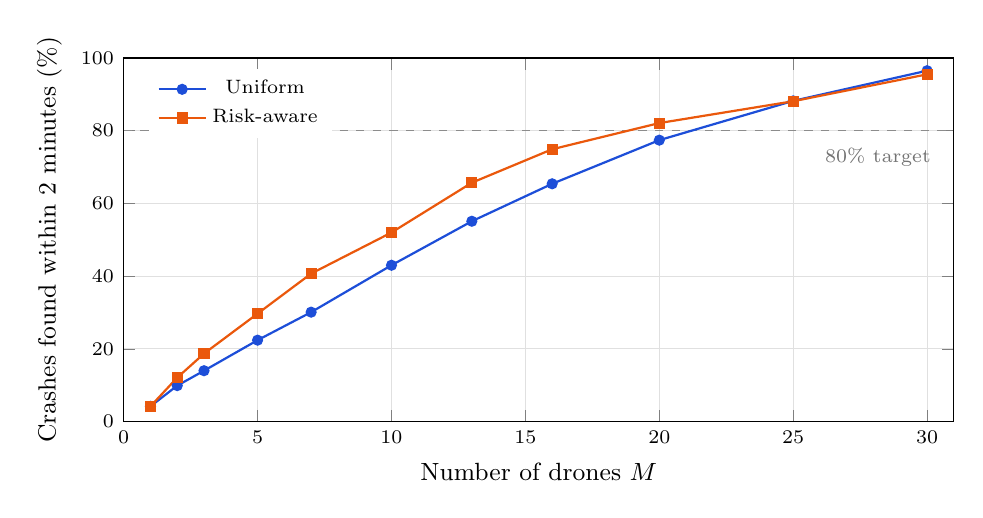
\begin{tikzpicture}
\begin{axis}[
  width=\linewidth, height=6.2cm,
  xlabel={Number of drones $M$},
  ylabel={Crashes found within 2 minutes (\%)},
  xlabel style={font=\small}, ylabel style={font=\small},
  ticklabel style={font=\scriptsize},
  xmin=0,xmax=31,ymin=0,ymax=100,
  grid=both, grid style={black!12},
  legend style={at={(0.03,0.97)},anchor=north west,draw=none,font=\scriptsize}]
\addplot[dashed,black!45,domain=0:31,forget plot] {80};
\node[font=\scriptsize,anchor=north east,text=black!55] at (axis cs:30.5,78)
  {80\% target};
\addplot[color=polUniform,mark=*,mark size=1.6pt,thick] coordinates
 {(1,4.2)(2,9.9)(3,14.0)(5,22.4)(7,30.1)(10,43.0)
  (13,55.1)(16,65.4)(20,77.4)(25,88.2)(30,96.5)};
\addplot[color=polRisk,mark=square*,mark size=1.6pt,thick] coordinates
 {(1,4.2)(2,12.1)(3,18.7)(5,29.7)(7,40.7)(10,52.0)
  (13,65.7)(16,74.9)(20,82.1)(25,88.1)(30,95.5)};
\legend{Uniform, Risk-aware}
\end{axis}
\end{tikzpicture}
\end{minipage}
\caption{Detection results by number of drones, from 50 trials of 30 days per
point. Both plans face the same crashes. Left: average alert time of the
crashes that were detected. Right: share of \emph{all} crashes detected within
two minutes, so missed crashes count against it.}
\label{fig:perf}
\end{figure}

\begin{table}[htbp]
\centering
\caption{Simulation results. Each row combines 50 trials of 30 simulated days,
about 1{,}800 crashes. The $\pm$ values are the standard errors of the average
alert time across trials.}
\label{tab:sweep}
\small
\begin{tabular}{@{}rrrrcrrr@{}}
\toprule
& \multicolumn{3}{c}{\textbf{Uniform}} & & \multicolumn{3}{c}{\textbf{Risk-aware}}\\
\cmidrule(lr){2-4}\cmidrule(lr){6-8}
$M$ & \textbf{Average $T$ (s)} & \textbf{Within 2 min} & \textbf{Missed} & & \textbf{Average $T$ (s)} & \textbf{Within 2 min} & \textbf{Missed} \\
\midrule
1  & $265.0\pm10.9$ & 4.2\%  & 83.9\% & & $265.0\pm10.9$ & 4.2\%  & 83.9\% \\
2  & $257.2\pm6.5$  & 9.9\%  & 66.7\% & & $253.5\pm6.2$  & 12.1\% & 61.7\% \\
3  & $252.9\pm6.2$  & 14.0\% & 54.1\% & & $245.1\pm5.7$  & 18.7\% & 44.8\% \\
5  & $245.1\pm5.1$  & 22.4\% & 29.0\% & & $210.7\pm4.1$  & 29.7\% & 22.1\% \\
7  & $226.5\pm4.3$  & 30.1\% & 11.9\% & & $168.1\pm3.9$  & 40.7\% & 14.1\% \\
10 & $176.6\pm3.5$  & 43.0\% & 0.2\%  & & $139.7\pm2.8$  & 52.0\% & 5.1\%  \\
13 & $124.8\pm2.3$  & 55.1\% & 0.0\%  & & $94.7\pm3.7$   & 65.7\% & 7.7\%  \\
16 & $93.4\pm2.0$   & 65.4\% & 0.0\%  & & $73.2\pm2.3$   & 74.9\% & 7.6\%  \\
20 & $66.4\pm1.8$   & 77.4\% & 0.0\%  & & $64.7\pm2.2$   & 82.1\% & 0.8\%  \\
25 & $45.6\pm1.0$   & 88.2\% & 0.0\%  & & $47.8\pm1.6$   & 88.1\% & 0.0\%  \\
30 & $31.2\pm0.9$   & 96.5\% & 0.0\%  & & $32.5\pm1.0$   & 95.5\% & 0.0\%  \\
\bottomrule
\end{tabular}
\end{table}

The risk-aware plan is faster whenever drones are scarce. The biggest gains are
in the middle of the range. With seven drones, the average alert time falls
from 226.5~s to 168.1~s, a 26\% cut. With ten drones, it falls from 176.6~s to
139.7~s, a 21\% cut. The standard errors here are only 2 to 4~s, so these
differences are far larger than random noise. Above about 25 drones the road is
well covered and the two plans give almost the same result: with 30 drones,
both are close to 32~s.

The two-minute share tells the same story in practical terms. To detect 80\% of
crashes within two minutes, the risk-aware plan needs about 19 drones and the
uniform plan about 21. Both plans reach 50\% at between 9 and 12 drones.

\subsection{The Distribution of Alert Time and the Coverage Trade-off}

Averages hide the most important result. The left side of Figure~\ref{fig:cdf}
shows, for ten drones, what share of crashes has been detected after each
number of seconds. The right side shows the missed share for every fleet size.

\begin{figure}[htbp]
\centering
\begin{minipage}[t]{0.48\textwidth}
\centering
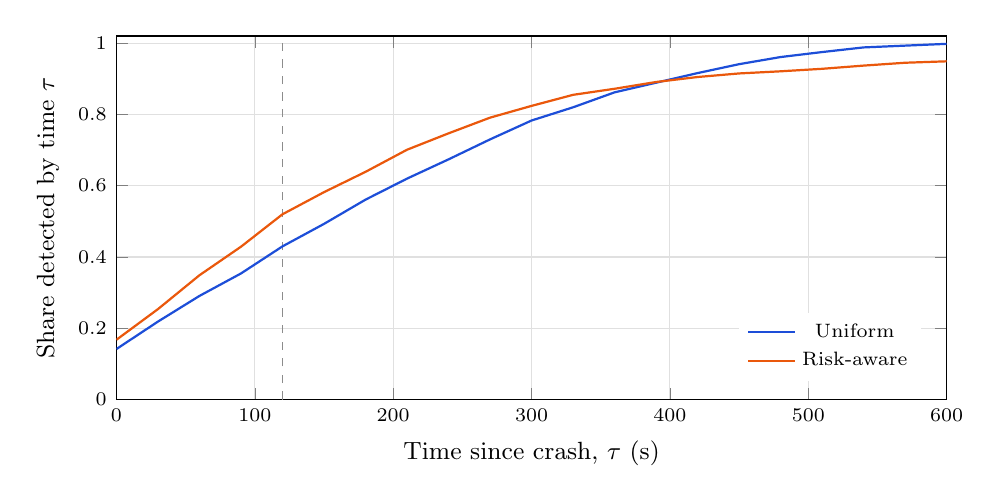
\begin{tikzpicture}
\begin{axis}[
  width=\linewidth, height=6.2cm,
  xlabel={Time since crash, $\tau$ (s)}, ylabel={Share detected by time $\tau$},
  xlabel style={font=\small}, ylabel style={font=\small},
  ticklabel style={font=\scriptsize},
  xmin=0,xmax=600,ymin=0,ymax=1.02,
  grid=both, grid style={black!12},
  legend style={at={(0.97,0.05)},anchor=south east,draw=none,font=\scriptsize}]
\addplot[dashed,black!45,forget plot] coordinates {(120,0)(120,1.02)};
\addplot[color=polUniform,thick,no marks] coordinates
 {(0,0.142)(30,0.219)(60,0.291)(90,0.354)(120,0.430)(150,0.493)(180,0.561)
  (210,0.620)(240,0.674)(270,0.730)(300,0.783)(330,0.820)(360,0.862)
  (390,0.889)(420,0.916)(450,0.941)(480,0.961)(510,0.975)(540,0.988)
  (570,0.993)(600,0.998)};
\addplot[color=polRisk,thick,no marks] coordinates
 {(0,0.168)(30,0.254)(60,0.349)(90,0.429)(120,0.520)(150,0.582)(180,0.639)
  (210,0.701)(240,0.747)(270,0.791)(300,0.824)(330,0.855)(360,0.872)
  (390,0.891)(420,0.905)(450,0.915)(480,0.921)(510,0.928)(540,0.937)
  (570,0.945)(600,0.949)};
\legend{Uniform, Risk-aware}
\end{axis}
\end{tikzpicture}
\end{minipage}\hfill
\begin{minipage}[t]{0.48\textwidth}
\centering
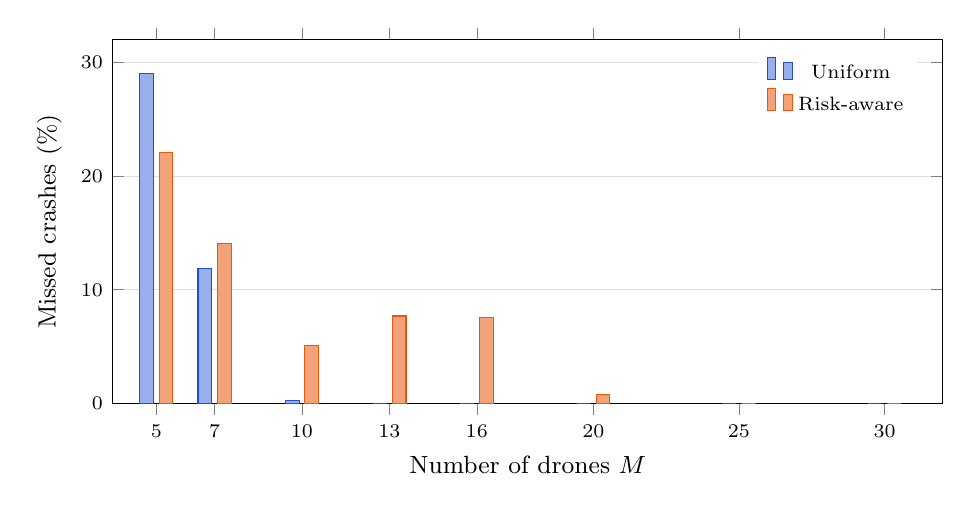
\begin{tikzpicture}
\begin{axis}[
  width=\linewidth, height=6.2cm,
  ybar, bar width=5pt,
  xlabel={Number of drones $M$}, ylabel={Missed crashes (\%)},
  xlabel style={font=\small}, ylabel style={font=\small},
  ticklabel style={font=\scriptsize},
  xmin=3.5,xmax=32,ymin=0,ymax=32,
  xtick={5,7,10,13,16,20,25,30},
  ymajorgrids, grid style={black!12},
  legend style={at={(0.97,0.97)},anchor=north east,draw=none,font=\scriptsize}]
\addplot[draw=polUniform,fill=polUniform!45] coordinates
 {(5,29.01)(7,11.91)(10,0.23)(13,0.00)(16,0.00)(20,0.00)(25,0.00)(30,0.00)};
\addplot[draw=polRisk,fill=polRisk!55] coordinates
 {(5,22.09)(7,14.07)(10,5.13)(13,7.69)(16,7.55)(20,0.80)(25,0.00)(30,0.00)};
\legend{Uniform, Risk-aware}
\end{axis}
\end{tikzpicture}
\end{minipage}
\caption{Left: share of crashes detected by each time, with ten drones. The
dashed line marks two minutes. The risk-aware plan is ahead until about 390~s;
after that the uniform plan catches up and ends higher. Right: share of crashes
not detected within 600~s. The uniform plan misses none from 13 drones on; the
risk-aware plan still misses 7.7\% at 13 drones.}
\label{fig:cdf}
\end{figure}

The two curves cross. Up to about 390~s, the risk-aware plan has detected more
crashes at every moment. After that, the uniform plan catches up and ends at
99.8\%, against 94.9\% for the risk-aware plan. With 13 and 16 drones, the
uniform plan misses no crashes at all, while the risk-aware plan misses 7.7\%
and 7.6\%.

The reason is segment length. A drone needs $2\ell/v$ seconds to fly the full
length $\ell$ of its segment and back. For this to fit inside the 600~s window
at 8~m/s, a segment can be at most $v\,T_{\max}/2 = 2.4$~km long.
Table~\ref{tab:longest} compares this limit with the longest segment in each
plan. Uniform segments are shorter than 2.4~km from 12 drones on, and from 13
drones the uniform plan misses nothing. The risk-aware plan keeps a southern
segment longer than 2.4~km until 25 drones.

\begin{table}[htbp]
\centering
\caption{Longest patrol segment and missed crashes. At 8~m/s, a drone can fly
at most 2.4~km and back within the 600~s window. Missed shares are from
Table~\ref{tab:sweep}.}
\label{tab:longest}
\small
\begin{tabular}{@{}rrlrr@{}}
\toprule
$M$ & \textbf{Uniform segment (km)} & \textbf{Longest risk-aware segment (km)} & \textbf{Missed, uniform} & \textbf{Missed, risk-aware} \\
\midrule
5  & 5.72 & 13.6 (15.0--28.6) & 29.0\% & 22.1\% \\
7  & 4.09 & 10.6 (18.0--28.6) & 11.9\% & 14.1\% \\
10 & 2.86 & 8.0 (20.0--28.0)  & 0.2\%  & 5.1\%  \\
13 & 2.20 & 9.6 (19.0--28.6)  & 0.0\%  & 7.7\%  \\
16 & 1.79 & 9.6 (19.0--28.6)  & 0.0\%  & 7.6\%  \\
20 & 1.43 & 4.0 (20.0--24.0)  & 0.0\%  & 0.8\%  \\
25 & 1.14 & 2.0 (12.0--14.0)  & 0.0\%  & 0.0\%  \\
30 & 0.95 & 1.0               & 0.0\%  & 0.0\%  \\
\bottomrule
\end{tabular}
\end{table}

Two things cause these long segments. First, the south is quiet: it has only
about 0.016 expected crashes per kilometre per day. So even a perfect
equal-load split with 13 drones (0.094 crashes per day each) would need
segments of about 6~km there. Second, the method gives the last segment
whatever is left over. With 13 and 16 drones, this leftover is 9.6~km, longer
than with 10 drones, which is why more crashes are missed with 13 and 16 drones
than with 10. With 10 drones, the same rule has the opposite effect: the last
segment is only 0.6~km long and carries 0.011 crashes per day, so one drone is
almost idle while its neighbour covers 8~km.

In short, for about 13 to 16 drones, the risk-aware plan gets a better average
and a better two-minute share by leaving a small number of crashes that it
effectively never covers.

\subsection{Sensitivity}
\label{sec:sensitivity}

Two settings have the largest effect. Figure~\ref{fig:sens} changes each of
them with ten drones, using 30 trials per point.

\begin{figure}[htbp]
\centering
\begin{minipage}[t]{0.48\textwidth}
\centering
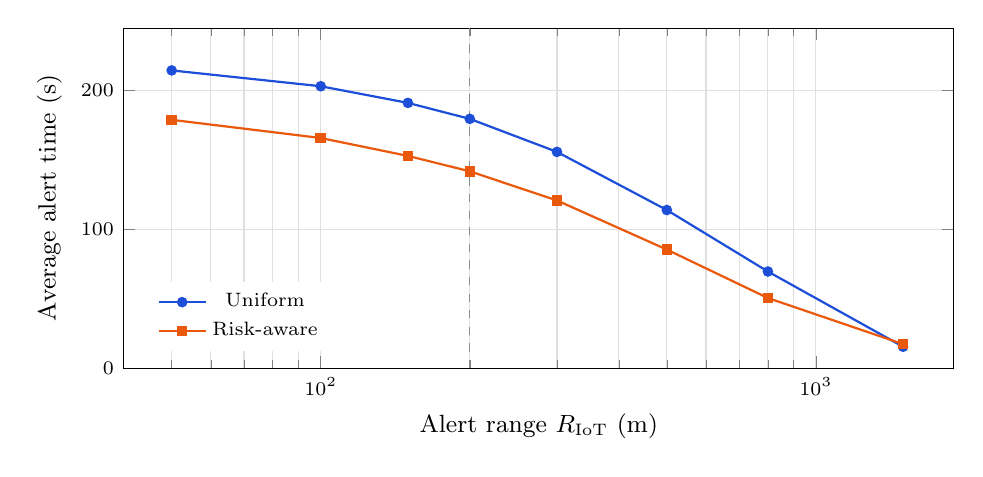
\begin{tikzpicture}
\begin{axis}[
  width=\linewidth, height=5.9cm,
  xlabel={Alert range $R_{\mathrm{IoT}}$ (m)}, ylabel={Average alert time (s)},
  xlabel style={font=\small}, ylabel style={font=\small},
  ticklabel style={font=\scriptsize},
  xmode=log, log basis x=10,
  xmin=40,xmax=1900,ymin=0,ymax=245,
  grid=both, grid style={black!12},
  legend style={at={(0.03,0.05)},anchor=south west,draw=none,font=\scriptsize}]
\addplot[dashed,black!45,forget plot] coordinates {(200,0)(200,245)};
\addplot[color=polUniform,mark=*,mark size=1.5pt,thick] coordinates
 {(50,214.6)(100,203.2)(150,191.2)(200,179.7)(300,155.9)
  (500,114.0)(800,69.7)(1500,15.5)};
\addplot[color=polRisk,mark=square*,mark size=1.5pt,thick] coordinates
 {(50,179.0)(100,165.9)(150,153.0)(200,141.9)(300,120.9)
  (500,85.5)(800,50.6)(1500,17.4)};
\legend{Uniform, Risk-aware}
\end{axis}
\end{tikzpicture}
\end{minipage}\hfill
\begin{minipage}[t]{0.48\textwidth}
\centering
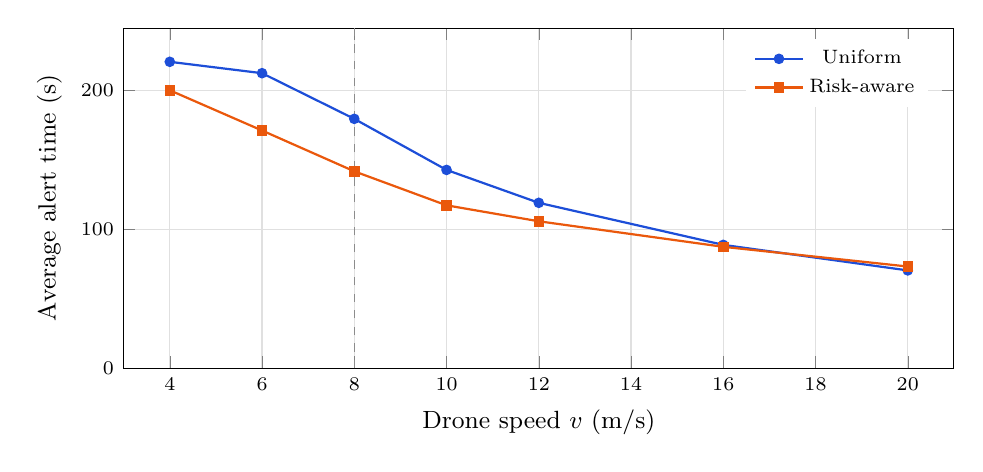
\begin{tikzpicture}
\begin{axis}[
  width=\linewidth, height=5.9cm,
  xlabel={Drone speed $v$ (m/s)}, ylabel={Average alert time (s)},
  xlabel style={font=\small}, ylabel style={font=\small},
  ticklabel style={font=\scriptsize},
  xmin=3,xmax=21,ymin=0,ymax=245,
  grid=both, grid style={black!12},
  legend style={at={(0.97,0.97)},anchor=north east,draw=none,font=\scriptsize}]
\addplot[dashed,black!45,forget plot] coordinates {(8,0)(8,245)};
\addplot[color=polUniform,mark=*,mark size=1.5pt,thick] coordinates
 {(4,220.8)(6,212.6)(8,179.7)(10,142.9)(12,119.2)(16,88.9)(20,70.5)};
\addplot[color=polRisk,mark=square*,mark size=1.5pt,thick] coordinates
 {(4,200.3)(6,171.3)(8,141.9)(10,117.4)(12,105.9)(16,87.5)(20,73.3)};
\legend{Uniform, Risk-aware}
\end{axis}
\end{tikzpicture}
\end{minipage}
\caption{Effect of changing one setting at a time, with ten drones and 30
trials per point. Left: alert range, on a logarithmic scale. Right: drone
speed. The dashed lines mark the default values. In both panels, the advantage
of the risk-aware plan disappears once the limit is relaxed far enough.}
\label{fig:sens}
\end{figure}

\paragraph{Alert Range.}
As the alert range grows, alert times fall, and the gap between the two plans
shrinks. At 200~m, the risk-aware plan is 38~s faster. At 800~m, it is still
19~s faster. At 1{,}500~m, the two plans are about the same (15.5~s against
17.4~s), and the risk-aware plan is even slightly slower. This confirms why we
chose 200~m (Section~\ref{sec:detection}): at the ranges a real LoRa radio can
reach, the alert zone covers so much of the road that the patrol plan hardly
matters. Comparing patrol plans at kilometre-scale alert ranges tells us almost
nothing.

\paragraph{Drone Speed.}
Speed shows the same pattern. At 4~m/s, the risk-aware plan is 20~s faster. At
8~m/s, it is 38~s faster. At 16~m/s, the two plans are equal, and at 20~m/s the
uniform plan is slightly ahead. A fast drone can cover a long segment quickly,
so putting more drones on busy stretches no longer pays off.

\paragraph{Battery and Docking.}
Turning off the battery model changes the average alert time by 2.7\% for the
uniform plan (184.6~s against 179.7~s) and by 8.5\% for the risk-aware plan
(129.9~s against 141.9~s). With ten drones, battery limits have only a small
effect, which is what the spare drones are designed to achieve.

\subsection{Time of Day}

Because the rates are real rates, the time of day now changes how many crashes
happen. When every hour of a 30-day trial uses the night rate, there are 26.7
crashes. When every hour uses the daytime rate, there are 42.6, which is 1.60
times as many. In the earlier score-based version, every time slot produced the
same number of crashes, so time of day only moved crashes from place to place.
This matters in practice: a fleet planned for night-time traffic would face
about 60\% more crashes during the day.

\subsection{Worked Example}
\label{sec:worked}

This example follows one crash through the system, using the application's own
code. We created three days of crashes from the rate table with a fixed seed
(20260921) and used the risk-aware plan for five drones
(Table~\ref{tab:segments}). To keep the example simple, every drone starts at
the northern end of its segment at midnight and moves as in
Equation~\ref{eq:motion}. We chose this crash because it shows why neighbouring
segments are tested; it is an example, not a random sample.

The crash happened on day 2 at 13:18, in section 3 (km 2--3) of the Khalde
region, at 2.869~km. The guardrail sensor there sends an alert that can be
received from 2.669 to 3.069~km. The crash lies in segment 1 (km 0--3), so the
drones tested are those in segments 1 and 2; there is no segment 0.

\begin{itemize}[leftmargin=*,itemsep=2pt]
\item The drone of segment 1 is at 0.647~km, flying north, away from the crash.
It must fly back to km~0 and then south to the alert zone, about 3.32~km in
total, which takes 414~s (case 3 of Equation~\ref{eq:cases}).
\item The drone of segment 2 is at 3.647~km, also flying north, which is towards
the alert zone. It is 0.578~km away, which takes 72~s (case 4).
\end{itemize}

The alert time is the shorter of the two, 72~s, so the crash is found by the
neighbouring drone, not by its own. Without testing the neighbour, this crash
would have waited almost seven minutes.

% ===========================================================================
\section{Discussion}
\label{sec:discussion}

\subsection{Interpretation of the Main Findings}

The most important finding about crashes is that roadside activity matters
most. The number of landmarks per kilometre explains more of the crash pattern
than road curves, ramps, traffic or speed. The reason makes sense. Where access
to the road is poorly controlled, roadside businesses cause cars to slow down,
turn and stop in the middle of fast traffic. These sudden speed differences are
known to cause collisions. On a motorway with strictly controlled access, this
factor would probably matter much less, which is the warning Elvik gives about
applying results from one place to another~\cite{elvik2013}.

The negative ramp result needs care. Three explanations fit the data. First,
regions with many ramps on this road may also be better designed, with bridges
instead of junctions, so ramp density may really measure road quality. Second,
ramps slow traffic down, and speed already has its own strong effect in the
model, so the ramp term may only capture what is left once speed is included.
Third, with only seven regions, a single unusual region can decide the sign.
We think the third explanation is the most likely, so we report the ramp result
as a pattern, not a cause. It is not evidence that ramps make roads safer.

The speed effect looks very large (rate ratio 20.3 per unit of $\ln S85$), but
it should be read with its wide confidence interval, 5.1 to 80.0, and the
narrow range of speeds it was measured over, 79 to 113~km/h. Within this range,
a 10\% higher speed means about 33\% more crashes, which is similar to other
studies. The result should not be used outside this range.

The model explains the difference between day and night through traffic alone,
without any separate term for the time of day. This is useful, because it means
the model can be used on other roads where traffic is measured. However, the
same property is why the model cannot tell the morning rush from the evening
rush: traffic and speed are similar in both, but the evening has twice as many
crashes. Something the data do not include, such as the direction of travel or
the purpose of the trip, must explain the difference.

\subsection{Why a Fitted Rate Model Changes the Swarm}

Replacing expert scores with fitted rates changed three things in the patrol
system. All three come from having real units, not from better numbers.

\emph{Drones moved north.} The expert scores gave the highest traffic score to
both ends of the road, because both ends are near towns. The crash records
disagree: the southern regions are the quietest on the road, with about one
sixth of the crash rate of the busiest. With five drones, two now cover the
first 6~km, while one covers the last 13.6~km.

\emph{Time of day now changes the number of crashes.} A score only shares out a
daily total among the time slots, so it cannot change how many crashes happen.
Real rates can, and they do: daytime has 1.6 times as many crashes as night.

\emph{The yearly total is now a result, not an assumption.} The earlier version
assumed 200 crashes per year. The model gives 446, more than twice as many. A
plan based on the old number would have been built for less than half of the
real workload.

\subsection{The Average-versus-Tail Trade-off}

The most useful result of this study is the one that does not favour the new
plan. Giving each drone an equal crash load balances the average. It treats a
drone covering 3~km in Khalde the same as a drone covering 13.6~km in the south,
because both expect the same number of crashes per day. In practice they are
very different. The southern drone takes longer than the detection window to
fly its segment and back, so a crash in its segment is not just found late; it
may never be found at all.

This is why, in the right panel of Figure~\ref{fig:cdf}, the uniform plan clearly
wins on missed crashes with 13 to 16 drones. Uniform segments are never longer
than $L/M$, which protects the worst case in a way the risk-aware plan does not.
The fix is not to drop the risk-aware plan but to limit it: no segment should
be longer than $v\,T_{\max}/2$ (2.4~km here), so that no drone is given more
road than it can cover in time. The equal-load rule would then work within this
limit. We did not add this limit here, because showing the trade-off as it is
tells the reader more than showing a patched version.

\subsection{Comparison with Previous Studies}

The model assumes that crashes rise in direct proportion to exposure. The data
suggest that they rise a little faster, with an elasticity of 1.33 (1.20 to
1.46), which matches earlier studies~\cite{lordmannering2010}. We kept the
simpler assumption because the patrol plan needs a rate per kilometre per hour,
and we accepted the small bias this causes.

Keeping the Poisson model goes against a common habit. Reviews note that crash
data often vary more than a Poisson model expects~\cite{lordmannering2010,
mannering2014}, and the raw counts here would suggest the same. But once the
risk factors are included, the leftover spread is close to 1. This supports a
point made by Cameron and Trivedi~\cite{cameron1990}: the test for extra
variation should be done after the model is fitted, not before.

On the drone side, research on multi-robot patrolling usually assumes that all
points are equally important~\cite{elmaliach2009,portugal2011}. Our results
suggest that weighting the patrol by a measured crash rate cuts the average
alert time by 21\% to 26\% when drones are scarce. They also show that this
weighting must respect how far a drone can fly in time, or it will miss crashes.
This problem does not appear in methods that treat all points as equal,
because in those methods it cannot happen.

\subsection{Implications}

\paragraph{For Research.}
On roads where access is poorly controlled, roadside activity should be
included as a main risk factor, not left out as background.

\paragraph{For Practice.}
A patrol system based on scores cannot be shown to be wrong. One based on rates
can: the regional and time-of-day checks in Section~\ref{sec:validation} can be
repeated every time the model is updated with new records. This is the
strongest reason for the change shown here, whatever the exact numbers are. For
planning, the results suggest that about 19 to 21 drones can detect 80\% of
crashes within two minutes on this 28.6~km road, with a 200~m alert range and a
speed of 8~m/s. Increasing the alert range of the guardrail sensors is a
cheaper way to improve detection than buying more drones.

\paragraph{For Policy.}
If roadside activity is the strongest factor, then managing road access should
come before changing the road's shape. This means fewer and combined entrances,
service roads, and control of roadside businesses. The finding that the old
assumption covered less than half of the real number of crashes also matters
for planning ambulance and emergency services on this road.

\subsection{Strengths and Limitations}

\paragraph{Strengths.}
A complete data table that keeps the cells with no crashes; a rule for choosing
the model that was fixed in advance; a total check that confirms the rate table
loses no crashes; a simulator that runs at the road's real crash rate; the same
crashes for both plans, for a fair comparison; and a record of the model terms
we tested and rejected.

\paragraph{Limitations of the Data.}
The main limits of this study come from its two datasets. The Lebanese Red
Cross records give the location of a crash only as a town name, so seven
regions is the most detail the data allow. For region features there are
therefore only seven independent values, every conclusion about location is
limited by this, and every 1~km section inside a region receives the same rate
because the data cannot tell them apart. The records also include only crashes
that an ambulance attended, so crashes with damage only are missing and the
real number of crashes is higher than the one modelled here. In addition, 908
records labelled with the city at the southern end of the road had no usable
location and were left out. The southern rates may therefore be too low, which
would make the risk-aware plan's long southern segment even more of a problem.
The CNRS-L GPS data carry their own limit: because the phone app lost users
over the study period, traffic could only be used as a relative level, and
removing this drop also removed real month-to-month changes in traffic.

\paragraph{Limitations of the Model.}
The model rests on simplifying assumptions that the data only partly support.
It assumes that crashes rise in proportion to exposure, while the data suggest
an elasticity of 1.33. It cannot separate the morning rush from the evening
rush, as Section~\ref{sec:validation} shows, because traffic and speed are
similar in both. Its rates are yearly averages, so the seasonal swing of about
1.38 between July and January is averaged out and the simulator has no
seasons. It does not model crash severity, so every simulated crash is treated
the same and the patrol plan cannot yet favour the most serious crashes. All
of its checks use the same data as the fit, because no crashes were kept aside
for testing. Finally, the study is observational: it shows patterns, not
causes.

\paragraph{Limitations of the Simulation.}
The detection model is idealised in three ways. First, it assumes that a
guardrail-mounted sensor is present at the exact point of every crash. In
practice, sensors would be fixed to the guardrail at set intervals, and some
crashes would happen between them or would not touch the guardrail at all.
Second, it assumes that the alert always gets through within
$R_{\mathrm{IoT}}$, with no lost messages, blocked signals or sensor failures.
It also assumes that a drone does not leave for the dock before it reaches the
crash, and the 5~s time step can make alert times up to one step too short.
Real alert times will therefore be longer than those reported here. Third, the
method that builds the risk-aware segments is uneven at the southern end: it
leaves a 0.6~km last segment with 10 drones and a 9.6~km one with 13 and 16
drones, and a more balanced splitting method would avoid this.

% ===========================================================================
\section{Conclusion}

This paper described a drone swarm system that detects road crashes on a
28.6~km motorway in Lebanon by picking up alerts from IoT sensors mounted on
the guardrail along the side of the road. At its centre, we replaced a
hand-made risk score with a crash-rate model fitted to two main datasets:
1{,}152 crashes attended by Lebanese Red Cross ambulances over 31 months, and
GPS traffic data from the \emph{tari2ak} smartphone application, obtained
through a collaboration with CNRS-L.

\paragraph{Main Findings.}
A useful crash-rate model can be built from records that give only a town name,
not an exact location. The model works at the level of seven regions and five
time slots; this limit is real but does not stop the model from being useful.
Roadside activity is the strongest risk factor, with a rate ratio of 3.84,
ahead of traffic, speed and road curves. The Poisson model fits well: the
leftover spread is 1.13, and the negative binomial improves the fit by only
3.4 AIC. The rates match the observed crash totals by region (correlation
0.990), but they cannot tell the two rush hours apart. In the simulator, the
risk-aware plan built on these rates cut the average alert time by 21\% to 26\%
with 7 to 16 drones. It reached the target of detecting 80\% of crashes within
two minutes with about 19 drones instead of 21. But for some fleet sizes it
left a long, quiet southern segment almost uncovered, and missed about 7.7\% of
crashes where the uniform plan missed none.

\paragraph{Scientific Contribution.}
The study shows three things. First, for crash modelling on a single road with
limited data, what limits the results most is how precisely the crash records
give locations, not how advanced the statistical method is. Second, even under
this limit, a fitted rate model is better than an expert score, mainly because
it can be checked against real data. Third, a drone patrol plan that follows
crash risk must also respect how far a drone can fly in time; otherwise it
trades a better average for crashes that are never found.

\paragraph{Recommendations for Future Work.}
We suggest five next steps. First, limit every risk-aware segment to
$v\,T_{\max}/2$ and repeat the comparison; we expect this to remove the missed
crashes without losing most of the gain in the average. Second, find the exact
location of a sample of crashes to test whether risk is really even within each
region. Third, model crash severity, so that the plan can favour the most
serious crashes. Fourth, install the hardware prototype on a real guardrail to
measure the alert range and delay, choose the spacing between sensors, and add
a realistic radio model with lost messages and blocked signals in place of the
perfect alert zone. Fifth, repeat the study on another road with strict access
control, to test whether roadside activity matters as much elsewhere.

% ===========================================================================
\section*{Code and Data Availability}

The source code of the Simulation-Aided Command Center, including the crash
generator, the patrol-segment builders, the alert-time model, the Monte Carlo
runner and the fitted rate table (\texttt{risk-table.json}) with its
coefficients, is openly available at
\url{https://github.com/hussein449/thesis_v2}~\cite{thesiscode}. The results in
this paper were produced with commit \texttt{ec8791a}. A live version of the
application runs in the web browser at
\url{https://thesis-tool.netlify.app/}~\cite{thesisapp}, where the reader can
run the patrol plans and the detection sweeps interactively. The raw ambulance
records belong to the Lebanese Red Cross, and the \emph{tari2ak} GPS data were
obtained through a collaboration with CNRS-L; neither dataset can be shared
publicly. For this reason, the data panel and the Python script that fits the
model are not included in the public repository.

% ===========================================================================
\begin{thebibliography}{99}
\small

\bibitem{who2023}
World Health Organization. \emph{Global Status Report on Road Safety 2023.}
WHO, Geneva, 2023.

\bibitem{sanchez2010}
R.~S\'anchez-Mangas, A.~Garc\'ia-Ferrer, A.~de~Juan, and A.~Mart\'in Arroyo.
\emph{The probability of death in road traffic accidents. How important is a
quick medical response?} Accident Analysis \& Prevention, 42(4):1048--1056,
2010.

\bibitem{byrne2019}
J.~P. Byrne, N.~C. Mann, M.~Dai, S.~A. Mason, P.~Karanicolas, S.~Rizoli, and
A.~B. Nathens. \emph{Association between emergency medical service response
time and motor vehicle crash mortality in the United States.} JAMA Surgery,
154(4):286--293, 2019.

\bibitem{elmaliach2009}
Y.~Elmaliach, N.~Agmon, and G.~A. Kaminka. \emph{Multi-robot area patrol under
frequency constraints.} Annals of Mathematics and Artificial Intelligence,
57(3--4):293--320, 2009.

\bibitem{portugal2011}
D.~Portugal and R.~Rocha. \emph{A survey on multi-robot patrolling algorithms.}
Technological Innovation for Sustainability, IFIP AICT 349, 139--146. Springer,
Berlin, 2011.

\bibitem{outay2020}
F.~Outay, H.~A. Mengash, and M.~Adnan. \emph{Applications of unmanned aerial
vehicle (UAV) in road safety, traffic and highway infrastructure management:
Recent advances and challenges.} Transportation Research Part A: Policy and
Practice, 141:116--129, 2020.

\bibitem{menouar2017}
H.~Menouar, I.~Guvenc, K.~Akkaya, A.~S. Uluagac, A.~Kadri, and A.~Tuncer.
\emph{UAV-enabled intelligent transportation systems for the smart city:
Applications and challenges.} IEEE Communications Magazine, 55(3):22--28, 2017.

\bibitem{washington2020}
S.~Washington, M.~G. Karlaftis, F.~Mannering, and P.~Anastasopoulos.
\emph{Statistical and Econometric Methods for Transportation Data Analysis,}
3rd edition. Chapman and Hall/CRC, Boca Raton, 2020.

\bibitem{lordmannering2010}
D.~Lord and F.~Mannering. \emph{The statistical analysis of crash-frequency
data: A review and assessment of methodological alternatives.} Transportation
Research Part A: Policy and Practice, 44(5):291--305, 2010.

\bibitem{miaou1994}
S.-P. Miaou. \emph{The relationship between truck accidents and geometric
design of road sections: Poisson versus negative binomial regressions.}
Accident Analysis \& Prevention, 26(4):471--482, 1994.

\bibitem{cameron1990}
A.~C. Cameron and P.~K. Trivedi. \emph{Regression-based tests for
overdispersion in the Poisson model.} Journal of Econometrics, 46(3):347--364,
1990.

\bibitem{lord2005}
D.~Lord, S.~P. Washington, and J.~N. Ivan. \emph{Poisson, Poisson-gamma and
zero-inflated regression models of motor vehicle crashes: Balancing statistical
fit and theory.} Accident Analysis \& Prevention, 37(1):35--46, 2005.

\bibitem{hsm2010}
American Association of State Highway and Transportation Officials.
\emph{Highway Safety Manual,} 1st edition. AASHTO, Washington, DC, 2010.

\bibitem{bonneson2012}
J.~Bonneson, S.~Geedipally, M.~P. Pratt, and D.~Lord. \emph{Safety Prediction
Methodology and Analysis Tool for Freeways and Interchanges.} NCHRP Project
17-45 Final Report, Transportation Research Board, Washington, DC, 2012.

\bibitem{park2010}
B.-J. Park, K.~Fitzpatrick, and D.~Lord. \emph{Evaluating the effects of
freeway design elements on safety.} Transportation Research Record,
2195:58--69, 2010.

\bibitem{hauer1997}
E.~Hauer. \emph{Observational Before--After Studies in Road Safety.} Pergamon,
Oxford, 1997.

\bibitem{elvik2013}
R.~Elvik. \emph{International transferability of accident modification
functions for horizontal curves.} Accident Analysis \& Prevention, 59:487--496,
2013.

\bibitem{mannering2014}
F.~L. Mannering and C.~R. Bhat. \emph{Analytic methods in accident research:
Methodological frontier and future directions.} Analytic Methods in Accident
Research, 1:1--22, 2014.

\bibitem{kanistras2013}
K.~Kanistras, G.~Martins, M.~J. Rutherford, and K.~P. Valavanis. \emph{A survey
of unmanned aerial vehicles (UAVs) for traffic monitoring.} International
Conference on Unmanned Aircraft Systems (ICUAS), 221--234, 2013.

\bibitem{mozaffari2019}
M.~Mozaffari, W.~Saad, M.~Bennis, Y.-H. Nam, and M.~Debbah. \emph{A tutorial
on UAVs for wireless networks: Applications, challenges, and open problems.}
IEEE Communications Surveys \& Tutorials, 21(3):2334--2360, 2019.

\bibitem{erdelj2017}
M.~Erdelj, E.~Natalizio, K.~R. Chowdhury, and I.~F. Akyildiz. \emph{Help from
the sky: Leveraging UAVs for disaster management.} IEEE Pervasive Computing,
16(1):24--32, 2017.

\bibitem{petajajarvi2015}
J.~Pet\"aj\"aj\"arvi, K.~Mikhaylov, A.~Roivainen, T.~H\"anninen, and
M.~Pettissalo. \emph{On the coverage of LPWANs: Range evaluation and channel
attenuation model for LoRa technology.} 14th International Conference on ITS
Telecommunications (ITST), Copenhagen, 2015.

\bibitem{vinodhini2025}
M.~Vinodhini, S.~Rajkumar, and S.~K. Subramaniam. \emph{Real-time Internet of
LoRa Things (IoLT)-based accident detection and prevention system in vehicular
networks towards smart city.} International Journal of Communication Systems,
38(1):e5692, 2025.

\bibitem{worldbank2017}
World Bank. \emph{Lebanon: Greater Beirut Public Transport Project.} Project
Appraisal Document, Project ID P160224, Washington, DC, 2017.

\bibitem{osm}
OpenStreetMap contributors. \emph{Planet dump.}
\texttt{https://planet.openstreetmap.org}, 2024. Open Database License,
\texttt{https://www.openstreetmap.org/copyright}.

\bibitem{hersbach2020}
H.~Hersbach, B.~Bell, P.~Berrisford, et al. \emph{The ERA5 global reanalysis.}
Quarterly Journal of the Royal Meteorological Society, 146(730):1999--2049,
2020.

\bibitem{balinski1982}
M.~L. Balinski and H.~P. Young. \emph{Fair Representation: Meeting the Ideal of
One Man, One Vote.} Yale University Press, New Haven, 1982.

\bibitem{seabold2010}
S.~Seabold and J.~Perktold. \emph{Statsmodels: Econometric and statistical
modeling with Python.} Proceedings of the 9th Python in Science Conference,
92--96, 2010.

\bibitem{knuth1997}
D.~E. Knuth. \emph{The Art of Computer Programming, Volume 2: Seminumerical
Algorithms,} 3rd edition. Addison-Wesley, Reading, MA, 1997.

\bibitem{mccullagh1989}
P.~McCullagh and J.~A. Nelder. \emph{Generalized Linear Models,} 2nd edition.
Chapman and Hall, London, 1989.

\bibitem{thesiscode}
H.~Nasereddine. \emph{Simulation-Aided Command Center: risk-driven UAV swarm
patrol simulator for the M51 corridor} [source code]. GitHub repository,
commit \texttt{ec8791a}, 2026. \url{https://github.com/hussein449/thesis_v2}
(accessed 22 September 2026).

\bibitem{thesisapp}
H.~Nasereddine. \emph{Simulation-Aided Command Center} [web application].
2026. \url{https://thesis-tool.netlify.app/} (accessed 22 September 2026).

\end{thebibliography}

\end{document}
